\documentclass[10pt,aspectratio=169]{beamer}

% --------------------------------------------------
% Idioma, tipografía y matemáticas
% --------------------------------------------------
\usepackage[utf8]{inputenc}
\usepackage[T1]{fontenc}
\usepackage[spanish,es-tabla]{babel}
\usepackage{lmodern}
\usepackage{amsmath,amssymb,mathtools}
\usepackage{graphicx}
\usepackage{svg}
\usepackage{xcolor}
\usepackage{hyperref}
\usepackage{tikz}
\usetikzlibrary{arrows.meta,positioning,calc,shapes.geometric,decorations.pathreplacing,decorations.pathmorphing,shadows}
\svgsetup{inkscapelatex=false}

% Si existe una conversión PDF del SVG, se usa para compilar sin Inkscape.
% El SVG original permanece en images/figures/ y sigue siendo editable.
\newcommand{\vectorfigure}[2][]{%
  \IfFileExists{#2.pdf}{\includegraphics[#1]{#2.pdf}}{%
    \IfFileExists{#2.png}{\includegraphics[#1]{#2.png}}{\includesvg[#1]{#2}}}%
}

% --------------------------------------------------
% Identidad visual conservada de la presentación original
% --------------------------------------------------
\definecolor{UdeCBlue}{HTML}{223C6A}
\definecolor{SoftBlue}{HTML}{EEF3FA}
\definecolor{DarkGray}{HTML}{2E2E2E}
\definecolor{SoftGray}{HTML}{F7F8FA}
\definecolor{WarmGold}{HTML}{B77A19}
\definecolor{SoftGold}{HTML}{FFF7E6}
\definecolor{RegularGreen}{HTML}{2E7D5B}
\definecolor{ChaosRed}{HTML}{B24C4C}

\setbeamercolor{normal text}{fg=DarkGray,bg=white}
\setbeamercolor{frametitle}{fg=UdeCBlue,bg=white}
\setbeamercolor{title}{fg=UdeCBlue,bg=white}
\setbeamercolor{structure}{fg=UdeCBlue}
\setbeamercolor{alerted text}{fg=ChaosRed}
\setbeamertemplate{navigation symbols}{}
\setbeamertemplate{footline}{%
  \leavevmode\hbox{%
  \begin{beamercolorbox}[wd=.84\paperwidth,ht=2.3ex,dp=1.2ex,leftskip=1.2em]{author in head/foot}%
    \scriptsize ¿Cómo encontrar caos partiendo desde el Modelo Estándar?
  \end{beamercolorbox}%
  \begin{beamercolorbox}[wd=.16\paperwidth,ht=2.3ex,dp=1.2ex,center]{date in head/foot}%
    \scriptsize\insertframenumber/\inserttotalframenumber
  \end{beamercolorbox}}}
\setbeamertemplate{itemize item}{\color{UdeCBlue}$\blacktriangleright$}
\setbeamertemplate{itemize subitem}{\color{UdeCBlue}$\circ$}
\setbeamerfont{frametitle}{series=\bfseries,size=\Large}
\setbeamerfont{title}{series=\bfseries,size=\Large}
\setbeamerfont{subtitle}{size=\large}

% --------------------------------------------------
% Comandos
% --------------------------------------------------
\newcommand{\focus}[1]{\textbf{\textcolor{UdeCBlue}{#1}}}
\newcommand{\caution}[1]{\textbf{\textcolor{WarmGold}{#1}}}
\newcommand{\softbox}[1]{%
  \begin{center}\setlength{\fboxsep}{8pt}%
  \fcolorbox{UdeCBlue!20}{SoftBlue}{%
    \begin{minipage}{0.92\linewidth}\centering #1\end{minipage}}
  \end{center}}
\newcommand{\goldbox}[1]{%
  \begin{center}\setlength{\fboxsep}{7pt}%
  \fcolorbox{WarmGold!60}{SoftGold}{%
    \begin{minipage}{0.92\linewidth}\centering #1\end{minipage}}
  \end{center}}
\newcommand{\sourcebar}[1]{%
  \vfill\par{\tiny\color{black!62}\raggedright #1\par}}
\newcommand{\Lag}{\mathcal L}
\newcommand{\Ham}{\mathcal H}
\newcommand{\SU}{\mathrm{SU}}
\newcommand{\U}{\mathrm{U}}
\newcommand{\Tr}{\operatorname{Tr}}
\newcommand{\dd}{\mathrm d}
\newcommand{\ii}{\mathrm i}

\title{¿Cómo encontrar caos partiendo desde el Modelo Estándar?}
\subtitle{Una ruta desde campos gauge clásicos hasta un Hamiltoniano no lineal}
\author{José Ignacio Rosas Sepúlveda}
\institute{Sistemas Dinámicos e Introducción al Caos}
\date{Agosto de 2026}

\begin{document}

% --------------------------------------------------
% 1. Portada
% --------------------------------------------------
\begin{frame}[plain]
\begin{columns}[T,totalwidth=\textwidth]
\begin{column}{0.72\textwidth}
\vspace{1.30cm}
{\usebeamerfont{title}\usebeamercolor[fg]{title}\inserttitle\par}
\vspace{0.35cm}
{\usebeamerfont{subtitle}\insertsubtitle\par}
\vspace{0.82cm}
{\large \insertauthor\par}
\vspace{0.18cm}
{\small \insertinstitute\par}
\vspace{0.18cm}
{\small \insertdate\par}
\end{column}
\begin{column}{0.24\textwidth}
\vspace{0.55cm}
\begin{center}

\includegraphics[width=0.82\linewidth]{images/UdeC_logo_azul.png}\par
\vspace{0.18cm}
{\scriptsize Universidad de Concepción}\par
{\scriptsize Ciencias Físicas}
\end{center}
\end{column}
\end{columns}
\vfill
{\color{UdeCBlue}\rule{\textwidth}{0.8pt}}
\end{frame}

% --------------------------------------------------
% 2. Motivación humana
% --------------------------------------------------

% omito esto por que lo dire de forma verbal en la presentacion con la diapositiva del titulo :p

% --------------------------------------------------
% 2. Preguntas iniciales
% --------------------------------------------------
\begin{frame}[plain]
\only<1>{%
  \vspace{1.45cm}
  \begin{center}
    {\Huge\bfseries ¿Que entendemos por caos?\par}
    \vspace{0.20cm}
    {\Huge\bfseries ¿Que es el Modelo Estándar\footnote{de física de particulas por cierto :p}?\par}
    \vspace{0.75cm}
  \end{center}
}
\end{frame}

% ================================================================
% TRES DIAPOSITIVAS: EJEMPLO ILUSTRATIVO DE CAOS CLÁSICO
% Insertar después de las preguntas iniciales y antes del bloque dedicado
% al Modelo Estándar.
%
% Requiere \vectorfigure, TikZ y los colores UdeCBlue, DarkGray, WarmGold,
% RegularGreen, ChaosRed, SoftBlue y SoftGold del preámbulo principal.
% ================================================================

% Dibuja el doble péndulo en la posición inicial indicada por dos ángulos
% medidos en radianes desde la vertical hacia abajo.
\providecommand{\penduloinicial}[3]{%
\begin{tikzpicture}[>=Latex,scale=.95,transform shape]
  \coordinate (O) at (0,1.35);
  \coordinate (A) at
    ({1.08*sin(deg(#1))},{1.35-1.08*cos(deg(#1))});
  \coordinate (B) at
    ({1.08*sin(deg(#1))+1.08*sin(deg(#2))},
     {1.35-1.08*cos(deg(#1))-1.08*cos(deg(#2))});

  \draw[line width=1.0pt,DarkGray] (-.48,1.35)--(.48,1.35);
  \draw[dashed,UdeCBlue!42] (O)--(0,-1.15);
  \draw[dashed,UdeCBlue!42] (A)--++(0,-1.20);

  \fill[UdeCBlue] (O) circle (2.7pt);
  \draw[line width=2.2pt,UdeCBlue] (O)--(A);
  \fill[UdeCBlue] (A) circle (5.0pt);
  \draw[line width=2.2pt,UdeCBlue] (A)--(B);
  \fill[#3] (B) circle (5.5pt);

  \node[font=\scriptsize,UdeCBlue,anchor=east] at
    ({.54*sin(deg(#1))},{1.35-.54*cos(deg(#1))}) {$\theta_1(0)$};
  \node[font=\scriptsize,#3,anchor=west] at
    ({1.08*sin(deg(#1))+.54*sin(deg(#2))},
     {1.35-1.08*cos(deg(#1))-.54*cos(deg(#2))}) {$\theta_2(0)$};
  \node[font=\scriptsize,DarkGray,anchor=west] at (A) {$m_1$};
  \node[font=\scriptsize,DarkGray,anchor=west] at (B) {$m_2$};
\end{tikzpicture}%
}

% --------------------------------------------------
% 1/3. Mismo sistema: una región regular
% --------------------------------------------------
\begin{frame}{Ejemplo ilustrativo: el doble péndulo}
\centering
{\scriptsize
\begin{align*}
 (m_1+m_2)L_1\ddot\theta_1
 +m_2L_2\cos\Delta\,\ddot\theta_2
 +m_2L_2\sin\Delta\,\dot\theta_2^{,2}
 +(m_1+m_2)g\sin\theta_1 &=0,\\[-0.08cm]
 L_2\ddot\theta_2
 +L_1\cos\Delta\,\ddot\theta_1
 -L_1\sin\Delta\,\dot\theta_1^{,2}
 +g\sin\theta_2 &=0,
 \qquad \Delta=\theta_1-\theta_2 .
\end{align*}}
\vspace{-0.34cm}

\begin{columns}[c,totalwidth=\textwidth]
\begin{column}{0.22\textwidth}
\centering
\penduloinicial{0.25}{0.35}{RegularGreen}
\vspace{0.05cm}

{\scriptsize
$z_0^{(R)}=(0.25,0,0.35,0)$}

\vspace{0.10cm}
{\small\color{RegularGreen}\bfseries región regular}
\end{column}

\begin{column}{0.76\textwidth}
\centering
\vectorfigure[width=\linewidth,keepaspectratio]
  {images/figures/doble_pendulo_region_regular}
\end{column}
\end{columns}
\vspace{-0.11cm}

{\small Las perturbaciones pequeñas permanecen superpuestas;
la curva gris corresponde al cambio grande de $2\,\mathrm{rad}$.}
\end{frame}

% --------------------------------------------------
% 2/3. Misma ecuación: una región caótica
% --------------------------------------------------
\begin{frame}{La misma ecuación diferencial, otra región inicial}
\centering
{\small Mismos parámetros y misma ecuación diferencial determinista;
solo cambiamos la región donde fijamos $z(0)$.}
\vspace{0.12cm}

\begin{columns}[c,totalwidth=\textwidth]
\begin{column}{0.22\textwidth}
\centering
\penduloinicial{2.20}{0.40}{ChaosRed}
\vspace{0.05cm}

{\scriptsize
$z_0^{(C)}=(2.20,0,0.40,0)$}

\vspace{0.10cm}
{\small\color{ChaosRed}\bfseries región caótica}
\end{column}

\begin{column}{0.76\textwidth}
\centering
\vectorfigure[width=\linewidth,keepaspectratio]
  {images/figures/doble_pendulo_region_caotica}
\end{column}
\end{columns}
\vspace{-0.08cm}

{\small Las perturbaciones más pequeñas tardan más en distinguirse,
pero terminan produciendo trayectorias macroscópicamente diferentes.}
\end{frame}

% --------------------------------------------------
% 3/3. Definición operativa y diagnósticos numéricos
% --------------------------------------------------
\begin{frame}{¿Qué entenderemos por caos clásico?}
\vspace{-0.08cm}

{\small
\textbf{Órbita:} fijada una condición inicial $z_0$, las ecuaciones de movimiento
generan una trayectoria $z(t)$ en el espacio de fases.}

\vspace{0.12cm}

\begin{columns}[T,totalwidth=\textwidth]
\begin{column}{0.61\textwidth}
\centering
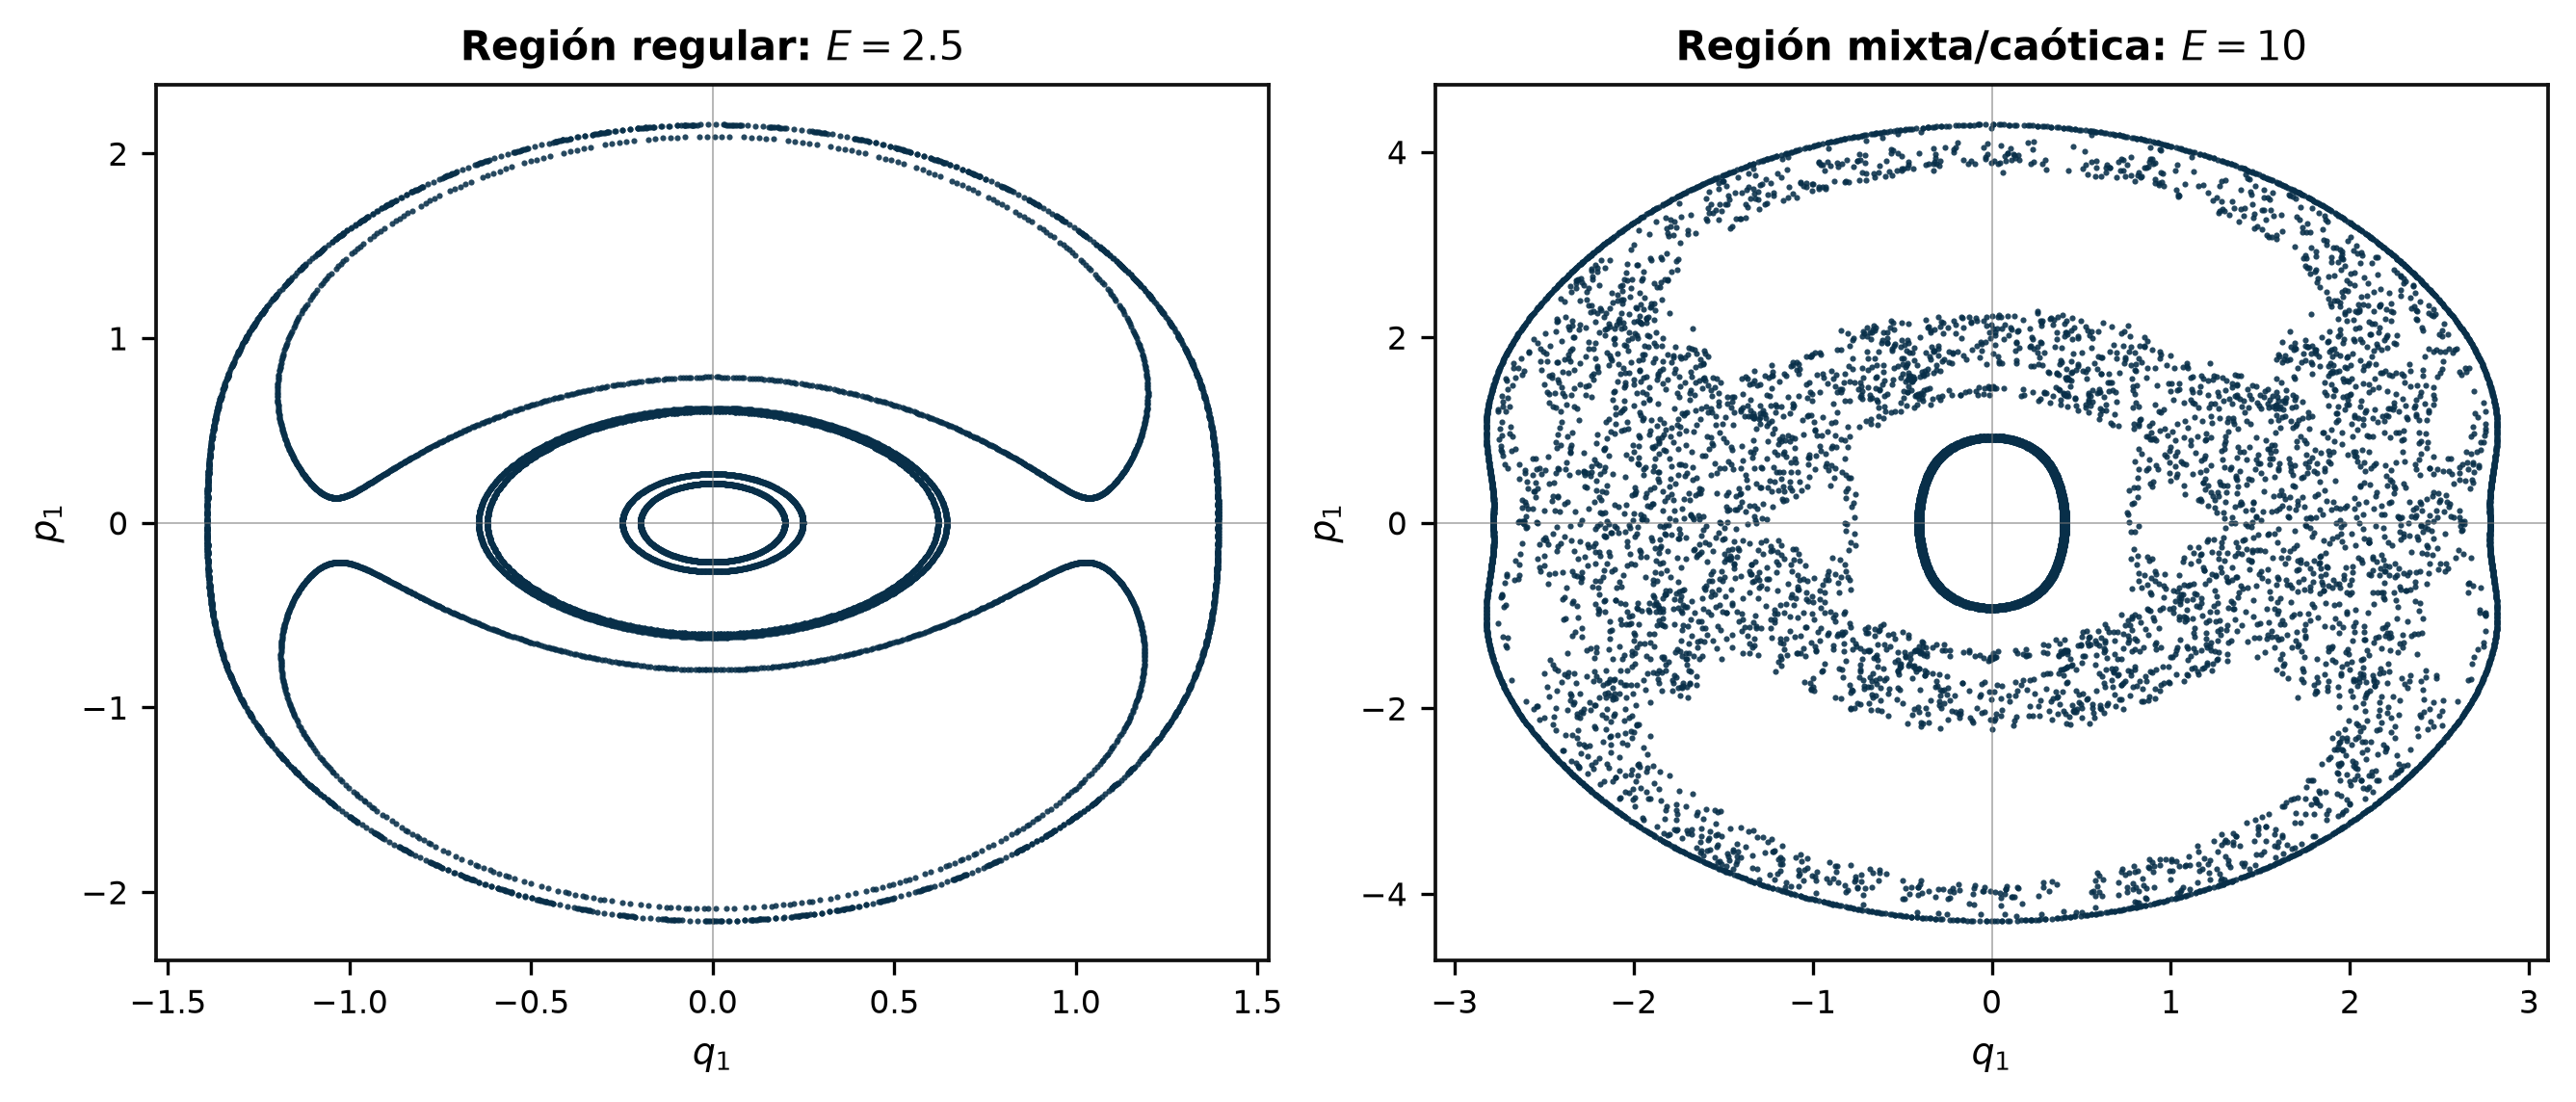
\includegraphics[width=\linewidth,height=4.55cm,keepaspectratio]
  {images/figures/poincare_intro_real.png}
\end{column}

\begin{column}{0.35\textwidth}
\vspace{0.18cm}
{\bfseries\color{UdeCBlue}Sección de Poincaré}

\vspace{0.10cm}
{\small
Elegimos una superficie transversal a la órbita y registramos
\textbf{solo los puntos donde la atraviesa}.}

\vspace{0.18cm}
\begin{itemize}\small
  \setlength\itemsep{0.18cm}
  \item curvas o islas $\rightarrow$ movimiento regular;
  \item puntos que llenan una región $\rightarrow$ comportamiento caótico o mixto.
\end{itemize}

\vspace{0.10cm}
{\scriptsize
En nuestro sistema, cambiar la condición inicial ---y en particular la energía---
puede llevarnos a regiones dinámicas distintas.}
\end{column}
\end{columns}
\end{frame}



% --------------------------------------------------
% 4a. Entrada popular y deliberadamente exagerada
% --------------------------------------------------
\begin{frame}{El Modelo Estándar...}
\centering
{\fontsize{24}{27}\selectfont\bfseries\color{WarmGold}
``¡LA PARTÍCULA DE DIOS!''}

\vspace{0.12cm}
{\small Higgs, colisiones de protones y la máquina más fotogénica de la física.}
\vspace{0.15cm}

\begin{tikzpicture}[x=1cm,y=1cm]
  % Fotografías reales, ligeramente inclinadas para dar una estética de
  % recorte periodístico. Los marcos conservan la paleta de la presentación.
  \node[rotate=-3,draw=UdeCBlue,line width=1.2pt,inner sep=2pt,fill=white]
    at (-4.05,0)
    {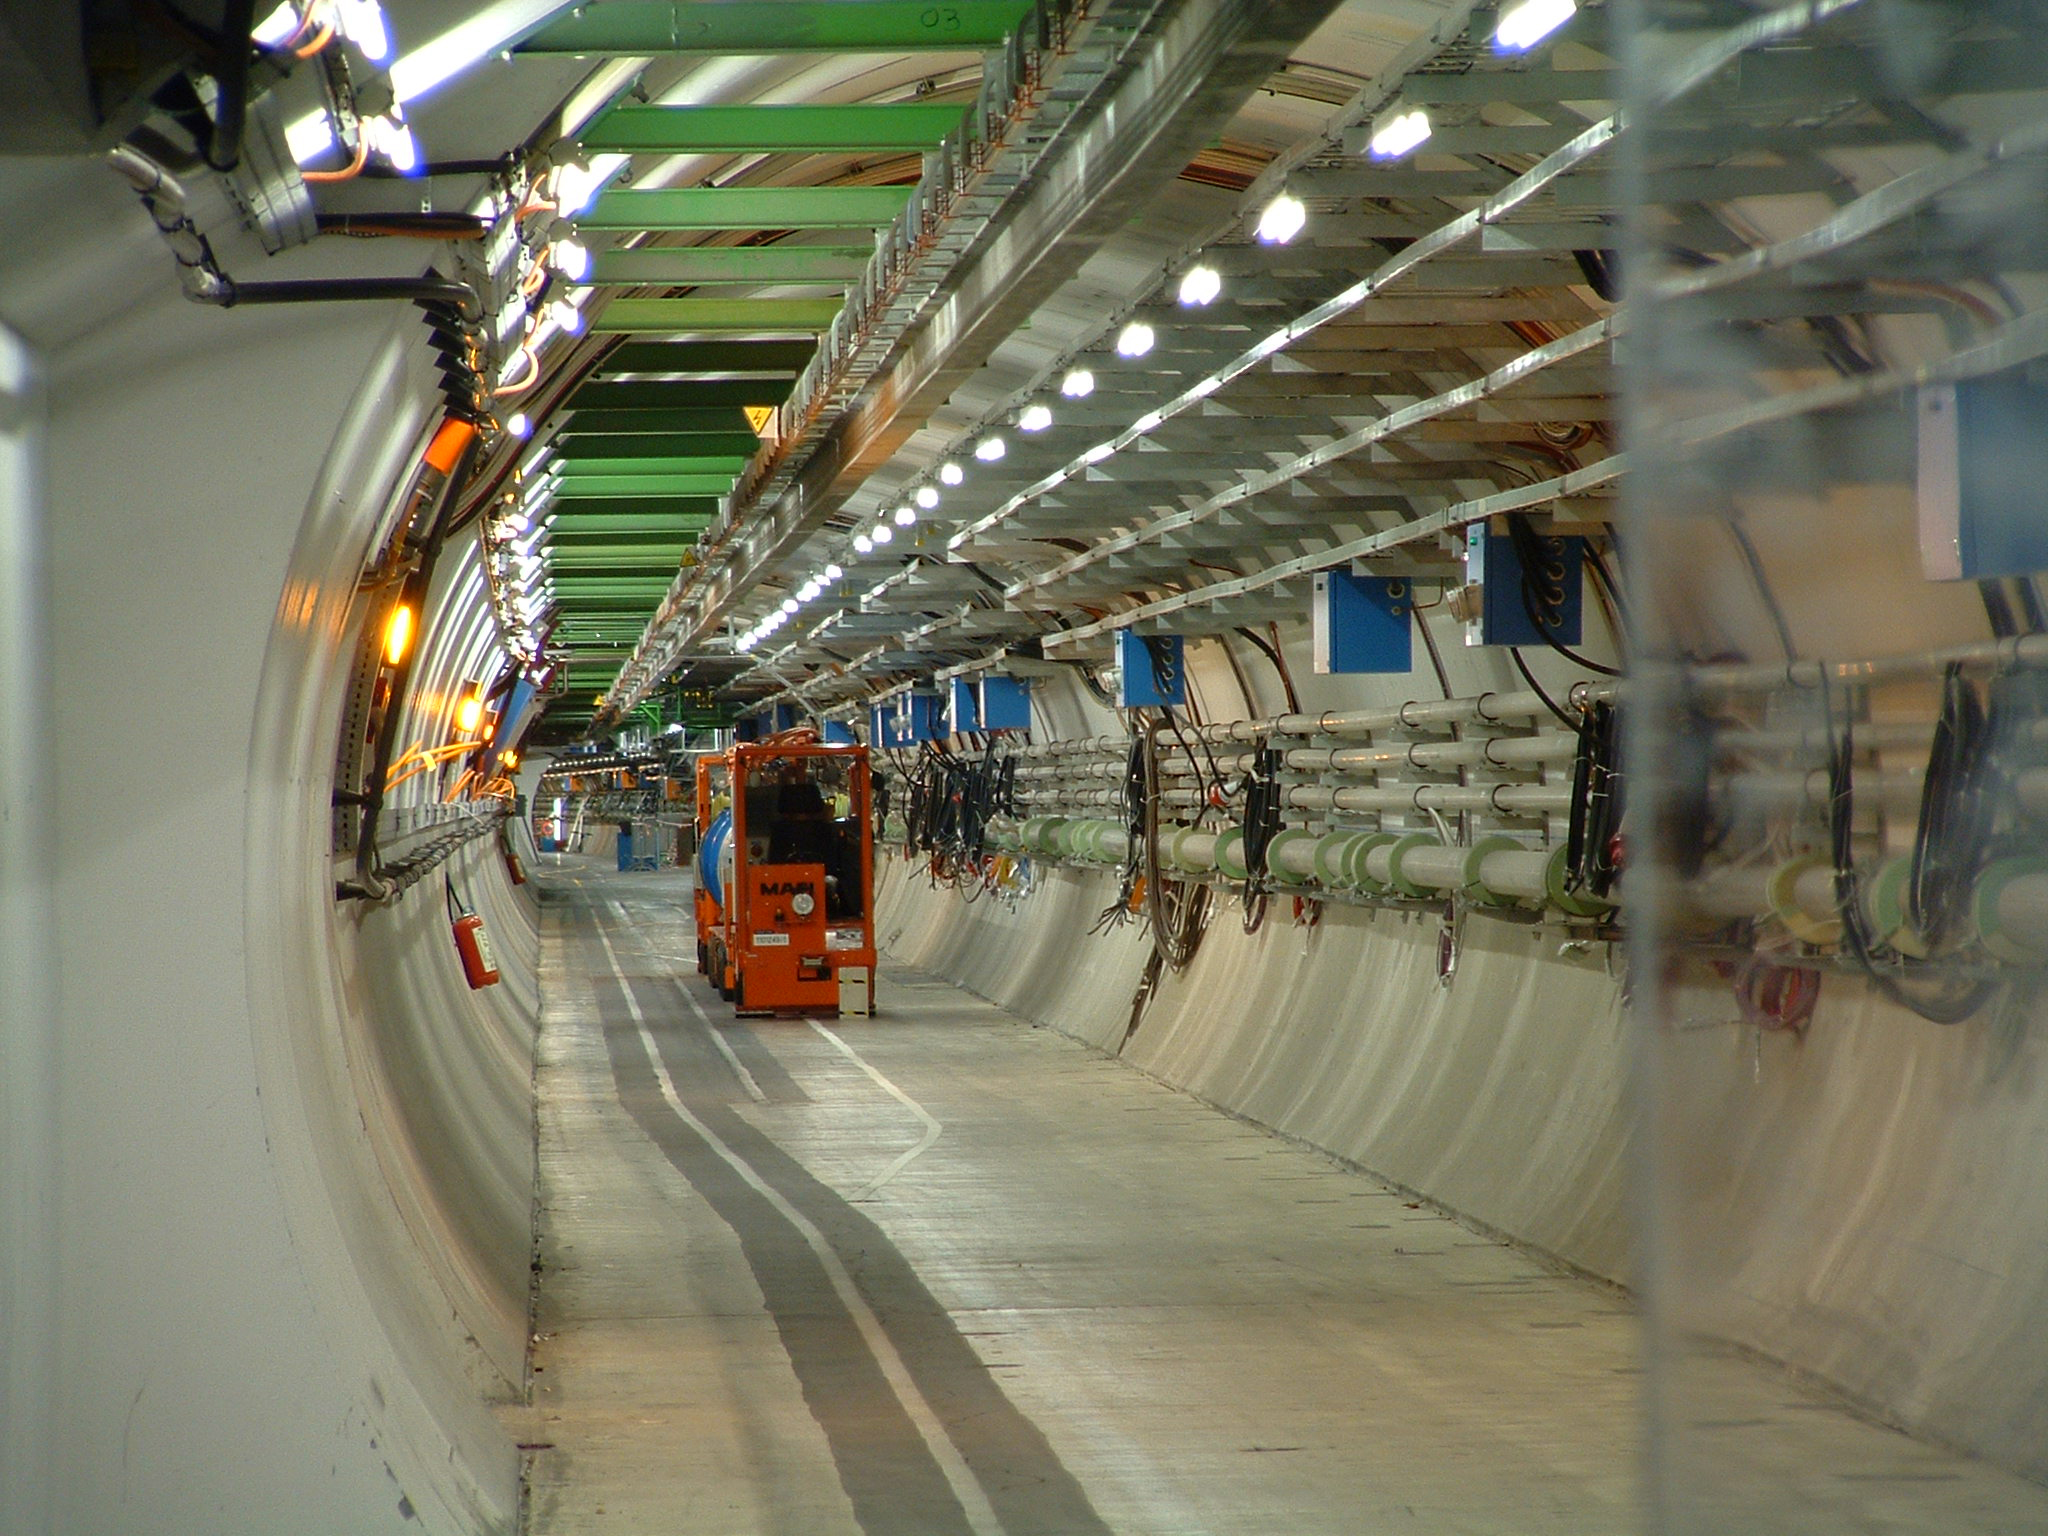
\includegraphics[width=3.45cm,height=3.05cm,keepaspectratio]
      {images/lhc_tunel.jpg}};
  \node[rotate=2,draw=WarmGold,line width=1.2pt,inner sep=2pt,fill=white]
    at (0,0)
    {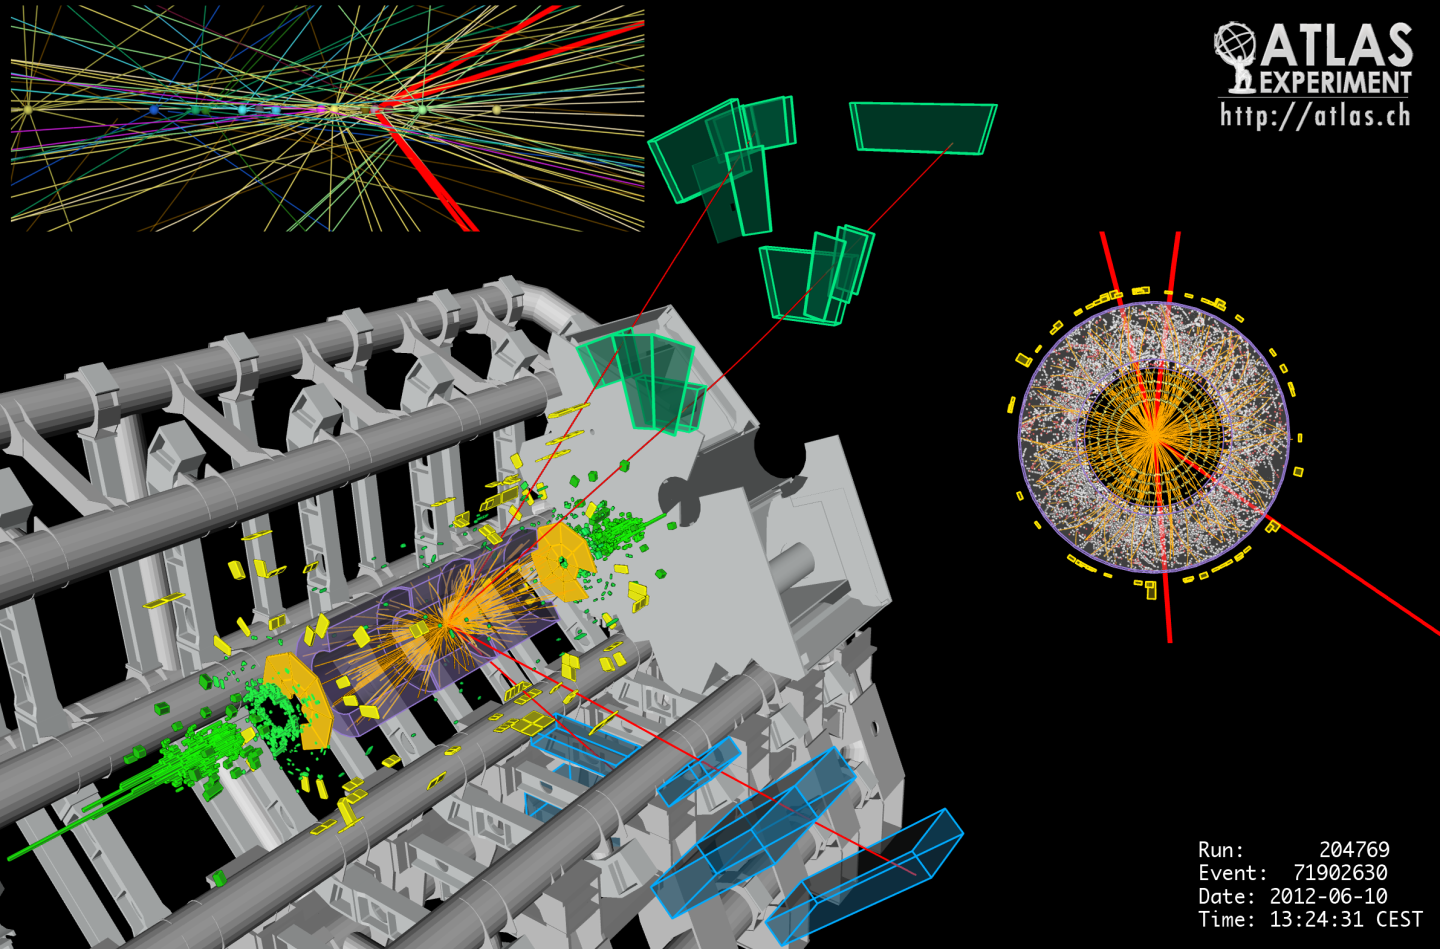
\includegraphics[width=3.70cm,height=3.05cm,keepaspectratio]
      {images/atlas_higgs_4mu.png}};
  \node[rotate=-2,draw=UdeCBlue,line width=1.2pt,inner sep=2pt,fill=white]
    at (4.05,0)
    {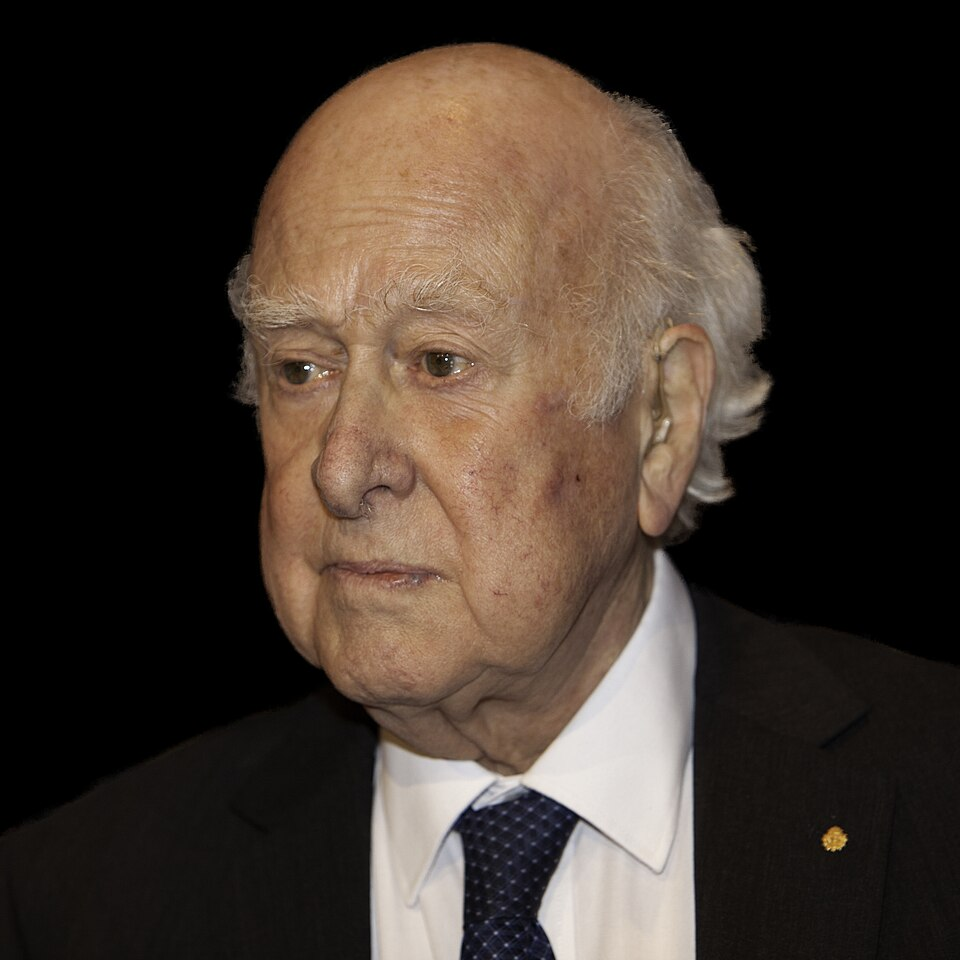
\includegraphics[width=3.20cm,height=3.05cm,keepaspectratio]
      {images/peter_higgs.jpg}};

  \node[fill=UdeCBlue,text=white,rounded corners=2pt,
        font=\scriptsize\bfseries,inner xsep=5pt,inner ysep=2.5pt]
        at (-4.05,-1.76) {27 km de acelerador};
  \node[fill=WarmGold,text=white,rounded corners=2pt,
        font=\scriptsize\bfseries,inner xsep=5pt,inner ysep=2.5pt]
        at (0,-1.76) {una colisión candidata a Higgs};
  \node[fill=UdeCBlue,text=white,rounded corners=2pt,
        font=\scriptsize\bfseries,inner xsep=5pt,inner ysep=2.5pt]
        at (4.05,-1.76) {Peter Higgs};
\end{tikzpicture}


\vspace{0.10cm}
{\large\color{UdeCBlue}\bfseries
Todo muy espectacular. Pero ¿qué clase de teoría es realmente?}

\sourcebar{El apodo ``God particle'' es popular, no un nombre técnico.
Imágenes: ATLAS/CERN, \href{https://commons.wikimedia.org/wiki/File:Event_display_of_a_4-muon_candidate_in_the_ATLAS_detector.png}{CC BY-SA 3.0};
Max Braun, \href{https://commons.wikimedia.org/wiki/File:LHC,_CERN.jpg}{CC BY-SA 2.0};
Bengt Nyman, \href{https://commons.wikimedia.org/wiki/File:Peter_W._Higgs_(50372668271).jpg}{CC BY 2.0}.}
\end{frame}

% --------------------------------------------------
% 4b. La tensión cuántica, ahora con la precisión conceptual
% --------------------------------------------------
\begin{frame}{Ahora sí: el Modelo Estándar es una teoría cuántica de campos}
\begin{columns}[T,totalwidth=\textwidth]
% --------------------------------------------------
% Mecánica clásica
% --------------------------------------------------
\begin{column}{0.46\textwidth}
\centering
{\large\bfseries\color{UdeCBlue}Mecánica clásica}

\vspace{0.10cm}
\begin{tikzpicture}[>=Latex,scale=.74,transform shape]
  \draw[->,DarkGray] (-2.25,0)--(2.35,0) node[right] {$q$};
  \draw[->,DarkGray] (0,-1.52)--(0,1.72) node[above] {$p$};
  \draw[very thick,UdeCBlue,smooth] plot coordinates
    {(-1.85,-1.15)(-1.30,-.56)(-.72,-.12)(-.18,.29)
     (.44,.70)(1.18,1.04)(1.92,1.30)};
  \foreach \x/\y/\lab in {-1.30/-.56/t_1,-.18/.29/t_2,1.18/1.04/t_3}{
    \fill[WarmGold] (\x,\y) circle (2.7pt);
    \node[font=\scriptsize,anchor=north west,WarmGold] at (\x+.05,\y-.04) {$\lab$};
  }
  \node[anchor=south east,UdeCBlue,font=\small] at (1.92,1.38)
        {$z(t)=(q(t),p(t))$};
\end{tikzpicture}

\vspace{-0.10cm}
{\scriptsize En cada instante, la trayectoria asigna simultáneamente una posición
y un momento definidos.}

\vspace{0.06cm}
\[
  z_0\quad\xrightarrow{\ \dot z=f(z)\ }\quad z(t).
\]
\end{column}

% --------------------------------------------------
% Teoría cuántica
% --------------------------------------------------
\begin{column}{0.50\textwidth}
\centering
{\large\bfseries\color{UdeCBlue}Teoría cuántica}

\vspace{0.10cm}
{\small
$
  \mathrm{i}\hbar\,\partial_t|\psi(t)\rangle
  =\widehat H|\psi(t)\rangle
  \qquad
  \text{(Schrödinger)}
$}
\vspace{0.05cm}

\begin{tikzpicture}[>=Latex,scale=.72,transform shape]
  % Flechas primero para que queden detrás de los estados y observables.
  \draw[->,very thick,UdeCBlue] (-.05,0)--(-1.75,-1.00);
  \draw[->,very thick,UdeCBlue] (.05,0)--(1.75,-1.00);

  \fill[SoftBlue] (0,.28) ellipse (1.42cm and .76cm);
  \draw[UdeCBlue,thick] (0,.28) ellipse (1.42cm and .76cm);
  \node[align=center] at (0,.28) {estado\\[-1pt]$|\psi(t)\rangle$};

  \node[draw=UdeCBlue,rounded corners=3pt,fill=white,
        minimum width=2.25cm,minimum height=.72cm,align=center]
        at (-1.78,-1.30) {observable $\widehat q$\\distribución $P(q)$};
  \node[draw=UdeCBlue,rounded corners=3pt,fill=white,
        minimum width=2.25cm,minimum height=.72cm,align=center]
        at (1.78,-1.30) {observable $\widehat p$\\distribución $P(p)$};
\end{tikzpicture}

\vspace{-0.14cm}
\[
  [\widehat q,\widehat p]=\mathrm{i}\hbar,
  \qquad
  \Delta q\,\Delta p\geq\frac{\hbar}{2}.
\]
\end{column}
\end{columns}

\vspace{-0.12cm}
\softbox{\scriptsize
La evolución del estado puede ser determinista y unitaria. La formulación
cuántica usual no proporciona una sucesión de puntos $(q(t),p(t))$
simultáneamente nítidos que forme una trayectoria clásica de la partícula.}

\sourcebar{La incertidumbre expresa una propiedad del estado cuántico, no solo
imperfección experimental. Una medición posterior se refiere al estado ya
modificado por la medición anterior. Véanse
\href{https://en.wikipedia.org/wiki/Uncertainty_principle}{Uncertainty principle},
\href{https://en.wikipedia.org/wiki/Measurement_in_quantum_mechanics}{Measurement in quantum mechanics} y
\href{https://en.wikipedia.org/wiki/Quantum_field_theory}{Quantum field theory}.}
\end{frame}


% --------------------------------------------------
% Giro narrativo
% --------------------------------------------------

\begin{frame}[plain]
\begin{center}
  {\huge\bfseries entonces... ¿tiene sentido preguntar por encontrar caos partiendo desde el Modelo Estándar?}
\end{center}
\end{frame}


% --------------------------------------------------
% 11. Dos rutas de cuantización
% --------------------------------------------------
\begin{frame}{Para llegar a la QFT, primero aparece una teoría clásica de campos}
\vspace{-0.05cm}
\begin{columns}[T,totalwidth=\textwidth]
\begin{column}{.48\textwidth}
\centering
{\bfseries Cuantización canónica}
\vspace{0.07cm}
\begin{tikzpicture}[>=Latex,node distance=.34cm]
\node[draw=UdeCBlue,rounded corners=3pt,fill=SoftBlue,text width=4.9cm,align=center] (L) {$\Lag(\Phi,\partial\Phi)$};
\node[draw=UdeCBlue,rounded corners=3pt,fill=white,text width=4.9cm,align=center,below=of L] (P) {$\Pi_A=\dfrac{\partial\Lag}{\partial\dot\Phi_A}$};
\node[draw=UdeCBlue,rounded corners=3pt,fill=white,text width=4.9cm,align=center,below=of P] (H) {$H=\displaystyle\int\dd^3x\,(\Pi_A\dot\Phi_A-\Lag)$};
\node[draw=WarmGold,rounded corners=3pt,fill=SoftGold,text width=4.9cm,align=center,below=of H] (Q) {$\Phi,\Pi,H\rightarrow\widehat\Phi,\widehat\Pi,\widehat H$};
\draw[->,thick,UdeCBlue] (L)--(P);\draw[->,thick,UdeCBlue] (P)--(H);\draw[->,thick,WarmGold] (H)--(Q);
\end{tikzpicture}
\vspace{0.08cm}
{\small aparece explícitamente $\Lag$.}
\end{column}
\begin{column}{.48\textwidth}
\centering
{\bfseries Integral de caminos de Feynman}
\vspace{0.07cm}
\begin{tikzpicture}[>=Latex,node distance=.55cm]
\node[draw=UdeCBlue,rounded corners=3pt,fill=SoftBlue,text width=4.9cm,align=center] (S) {$S[\Phi]=\displaystyle\int\dd^4x\,\Lag$};
\node[draw=WarmGold,rounded corners=3pt,fill=SoftGold,text width=4.9cm,minimum height=1.10cm,align=center,below=of S] (PI) {$\displaystyle\int\!\mathcal D\Phi\;e^{\ii S[\Phi]/\hbar}$};
\draw[->,thick,WarmGold] (S)--(PI);
\end{tikzpicture}
\vspace{0.15cm}
{\small aparece explícitamente la acción $S$.}
\end{column}
\end{columns}
\vspace{0.02cm}
\goldbox{\small $\Lag$ y $S$ son objetos clásicos. La estrategia de esta charla es \textbf{retroceder hasta ellos}, antes de cuantizar, y estudiar una reducción clásica.}
\sourcebar{Se muestran solo las dos ideas de cuantización necesarias para motivar el regreso a la acción clásica; la cuantización rigurosa de teorías gauge requiere pasos adicionales.}
\end{frame}



% --------------------------------------------------
% 12. Antecedentes
% --------------------------------------------------
\begin{frame}{Volver a campos clásicos y reducirlos tiene una larga historia}
\vspace{-0.10cm}
\centering
\begin{tikzpicture}[x=1cm,y=1cm]
  % El collage replica la estética de recortes/fotografías de la diapositiva del Higgs:
  % papel blanco, borde fuerte, ligera rotación y una etiqueta independiente.
  \node[rotate=-2.4,draw=UdeCBlue,line width=1.25pt,inner sep=2pt,fill=white,drop shadow]
    at (-4.05,1.38)
    {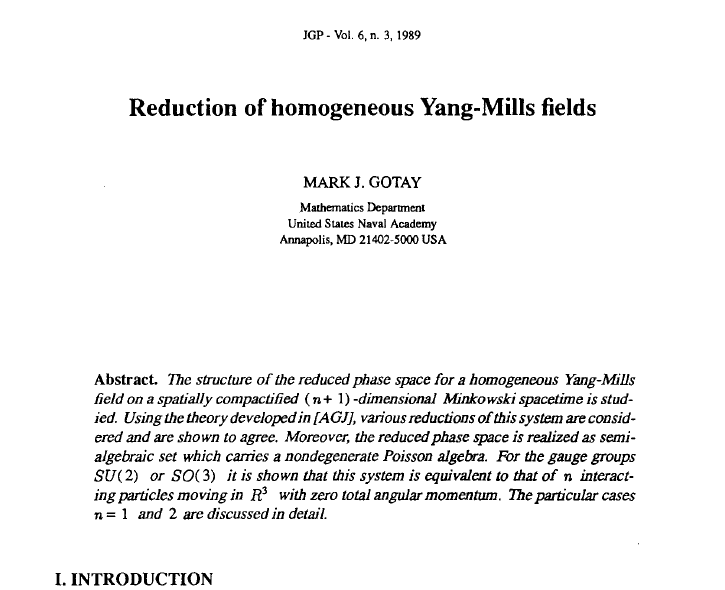
\includegraphics[width=3.30cm,height=2.34cm,keepaspectratio]{images/papers/paper_gotay_crop.png}};
  \node[rotate=1.8,draw=WarmGold,line width=1.25pt,inner sep=2pt,fill=white,drop shadow]
    at (0,1.38)
    {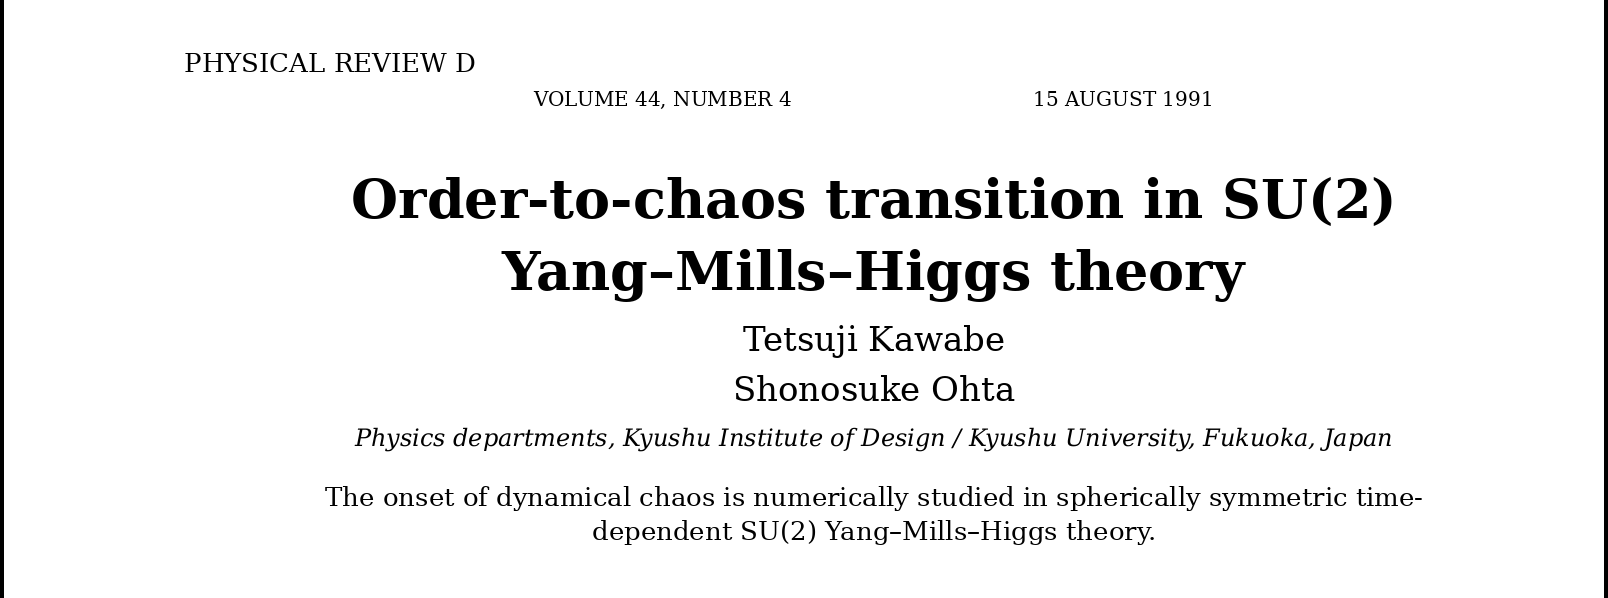
\includegraphics[width=3.30cm,height=2.34cm,keepaspectratio]{images/papers/paper_kawabe_crop.png}};
  \node[rotate=-1.8,draw=UdeCBlue,line width=1.25pt,inner sep=2pt,fill=white,drop shadow]
    at (4.05,1.38)
    {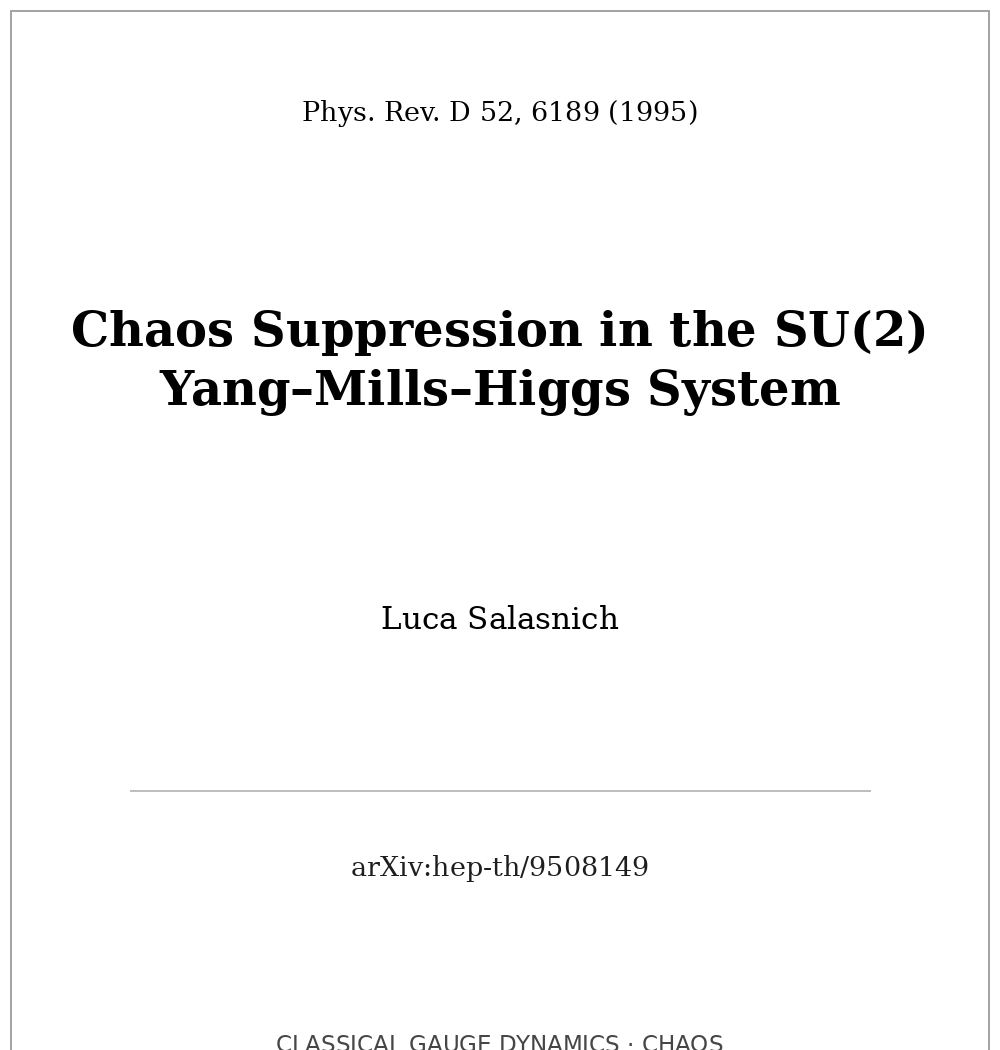
\includegraphics[width=3.30cm,height=2.34cm,keepaspectratio]{images/papers/paper_salasnich_crop.png}};

  \node[fill=UdeCBlue,text=white,rounded corners=2pt,
        font=\scriptsize\bfseries,inner xsep=5pt,inner ysep=2.5pt]
        at (-4.05,.02) {Gotay, 1989};
  \node[fill=WarmGold,text=white,rounded corners=2pt,
        font=\scriptsize\bfseries,inner xsep=5pt,inner ysep=2.5pt]
        at (0,.02) {Kawabe--Ohta, 1991};
  \node[fill=UdeCBlue,text=white,rounded corners=2pt,
        font=\scriptsize\bfseries,inner xsep=5pt,inner ysep=2.5pt]
        at (4.05,.02) {Salasnich, 1995};

  \node[rotate=2.0,draw=RegularGreen,line width=1.25pt,inner sep=2pt,fill=white,drop shadow]
    at (-2.18,-1.72)
    {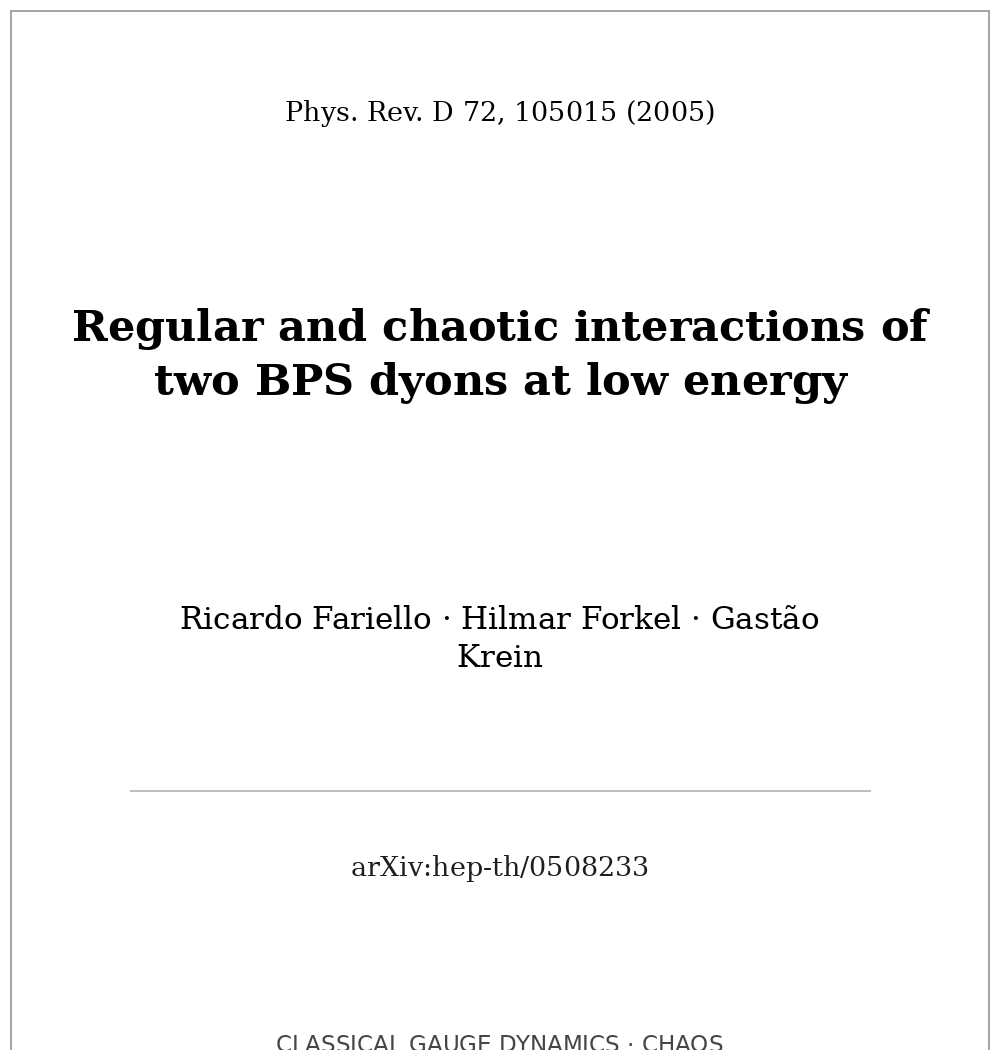
\includegraphics[width=3.55cm,height=2.18cm,keepaspectratio]{images/papers/paper_fariello_crop.png}};
  \node[rotate=-2.2,draw=ChaosRed,line width=1.25pt,inner sep=2pt,fill=white,drop shadow]
    at (2.18,-1.72)
    {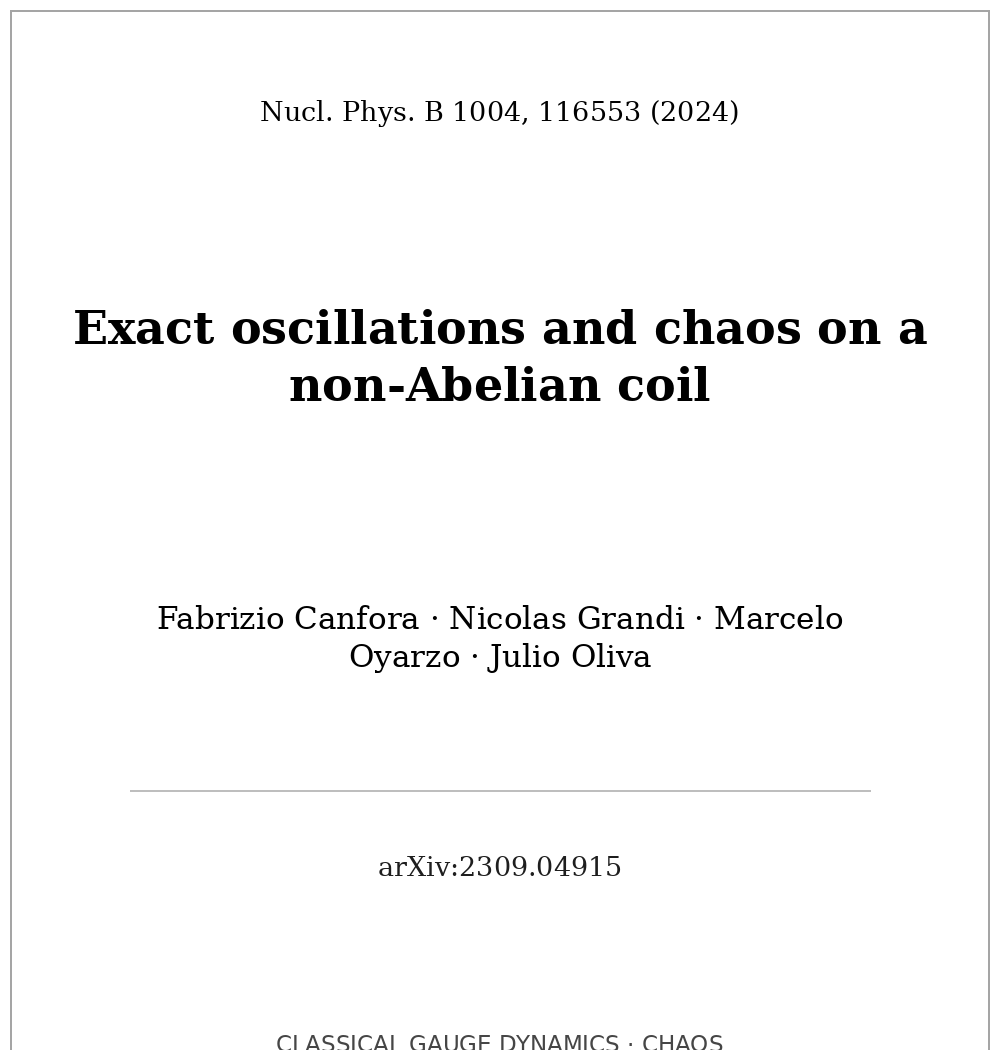
\includegraphics[width=3.72cm,height=2.18cm,keepaspectratio]{images/papers/paper_canfora_crop.png}};

  \node[fill=RegularGreen,text=white,rounded corners=2pt,
        font=\scriptsize\bfseries,inner xsep=5pt,inner ysep=2.5pt]
        at (-2.18,-3.02) {Fariello--Forkel--Krein, 2005};
  \node[fill=ChaosRed,text=white,rounded corners=2pt,
        font=\scriptsize\bfseries,inner xsep=5pt,inner ysep=2.5pt]
        at (2.18,-3.02) {Canfora--Grandi--Oyarzo--Oliva, 2024};
\end{tikzpicture}
\sourcebar{La literatura clásica de Yang--Mills y Yang--Mills--Higgs usa reducciones de pocos modos y secciones de Poincaré para estudiar regularidad y caos.}
\end{frame}

% --------------------------------------------------
% 12b. Un momento... :)
% --------------------------------------------------
{
\setbeamercolor{background canvas}{bg=black}
\begin{frame}[plain]
\begin{tikzpicture}[remember picture,overlay]
  % Título: el único texto de la diapositiva.
  \node[anchor=north west,text=white,font=\bfseries\Large]
    at ([xshift=.65cm,yshift=-.48cm]current page.north west) {Un momento...};

  % El meme queda integrado en las esquinas sobre fondo negro.
  \node[anchor=south west,inner sep=0pt]
    at ([xshift=-.12cm,yshift=-.10cm]current page.south west)
    {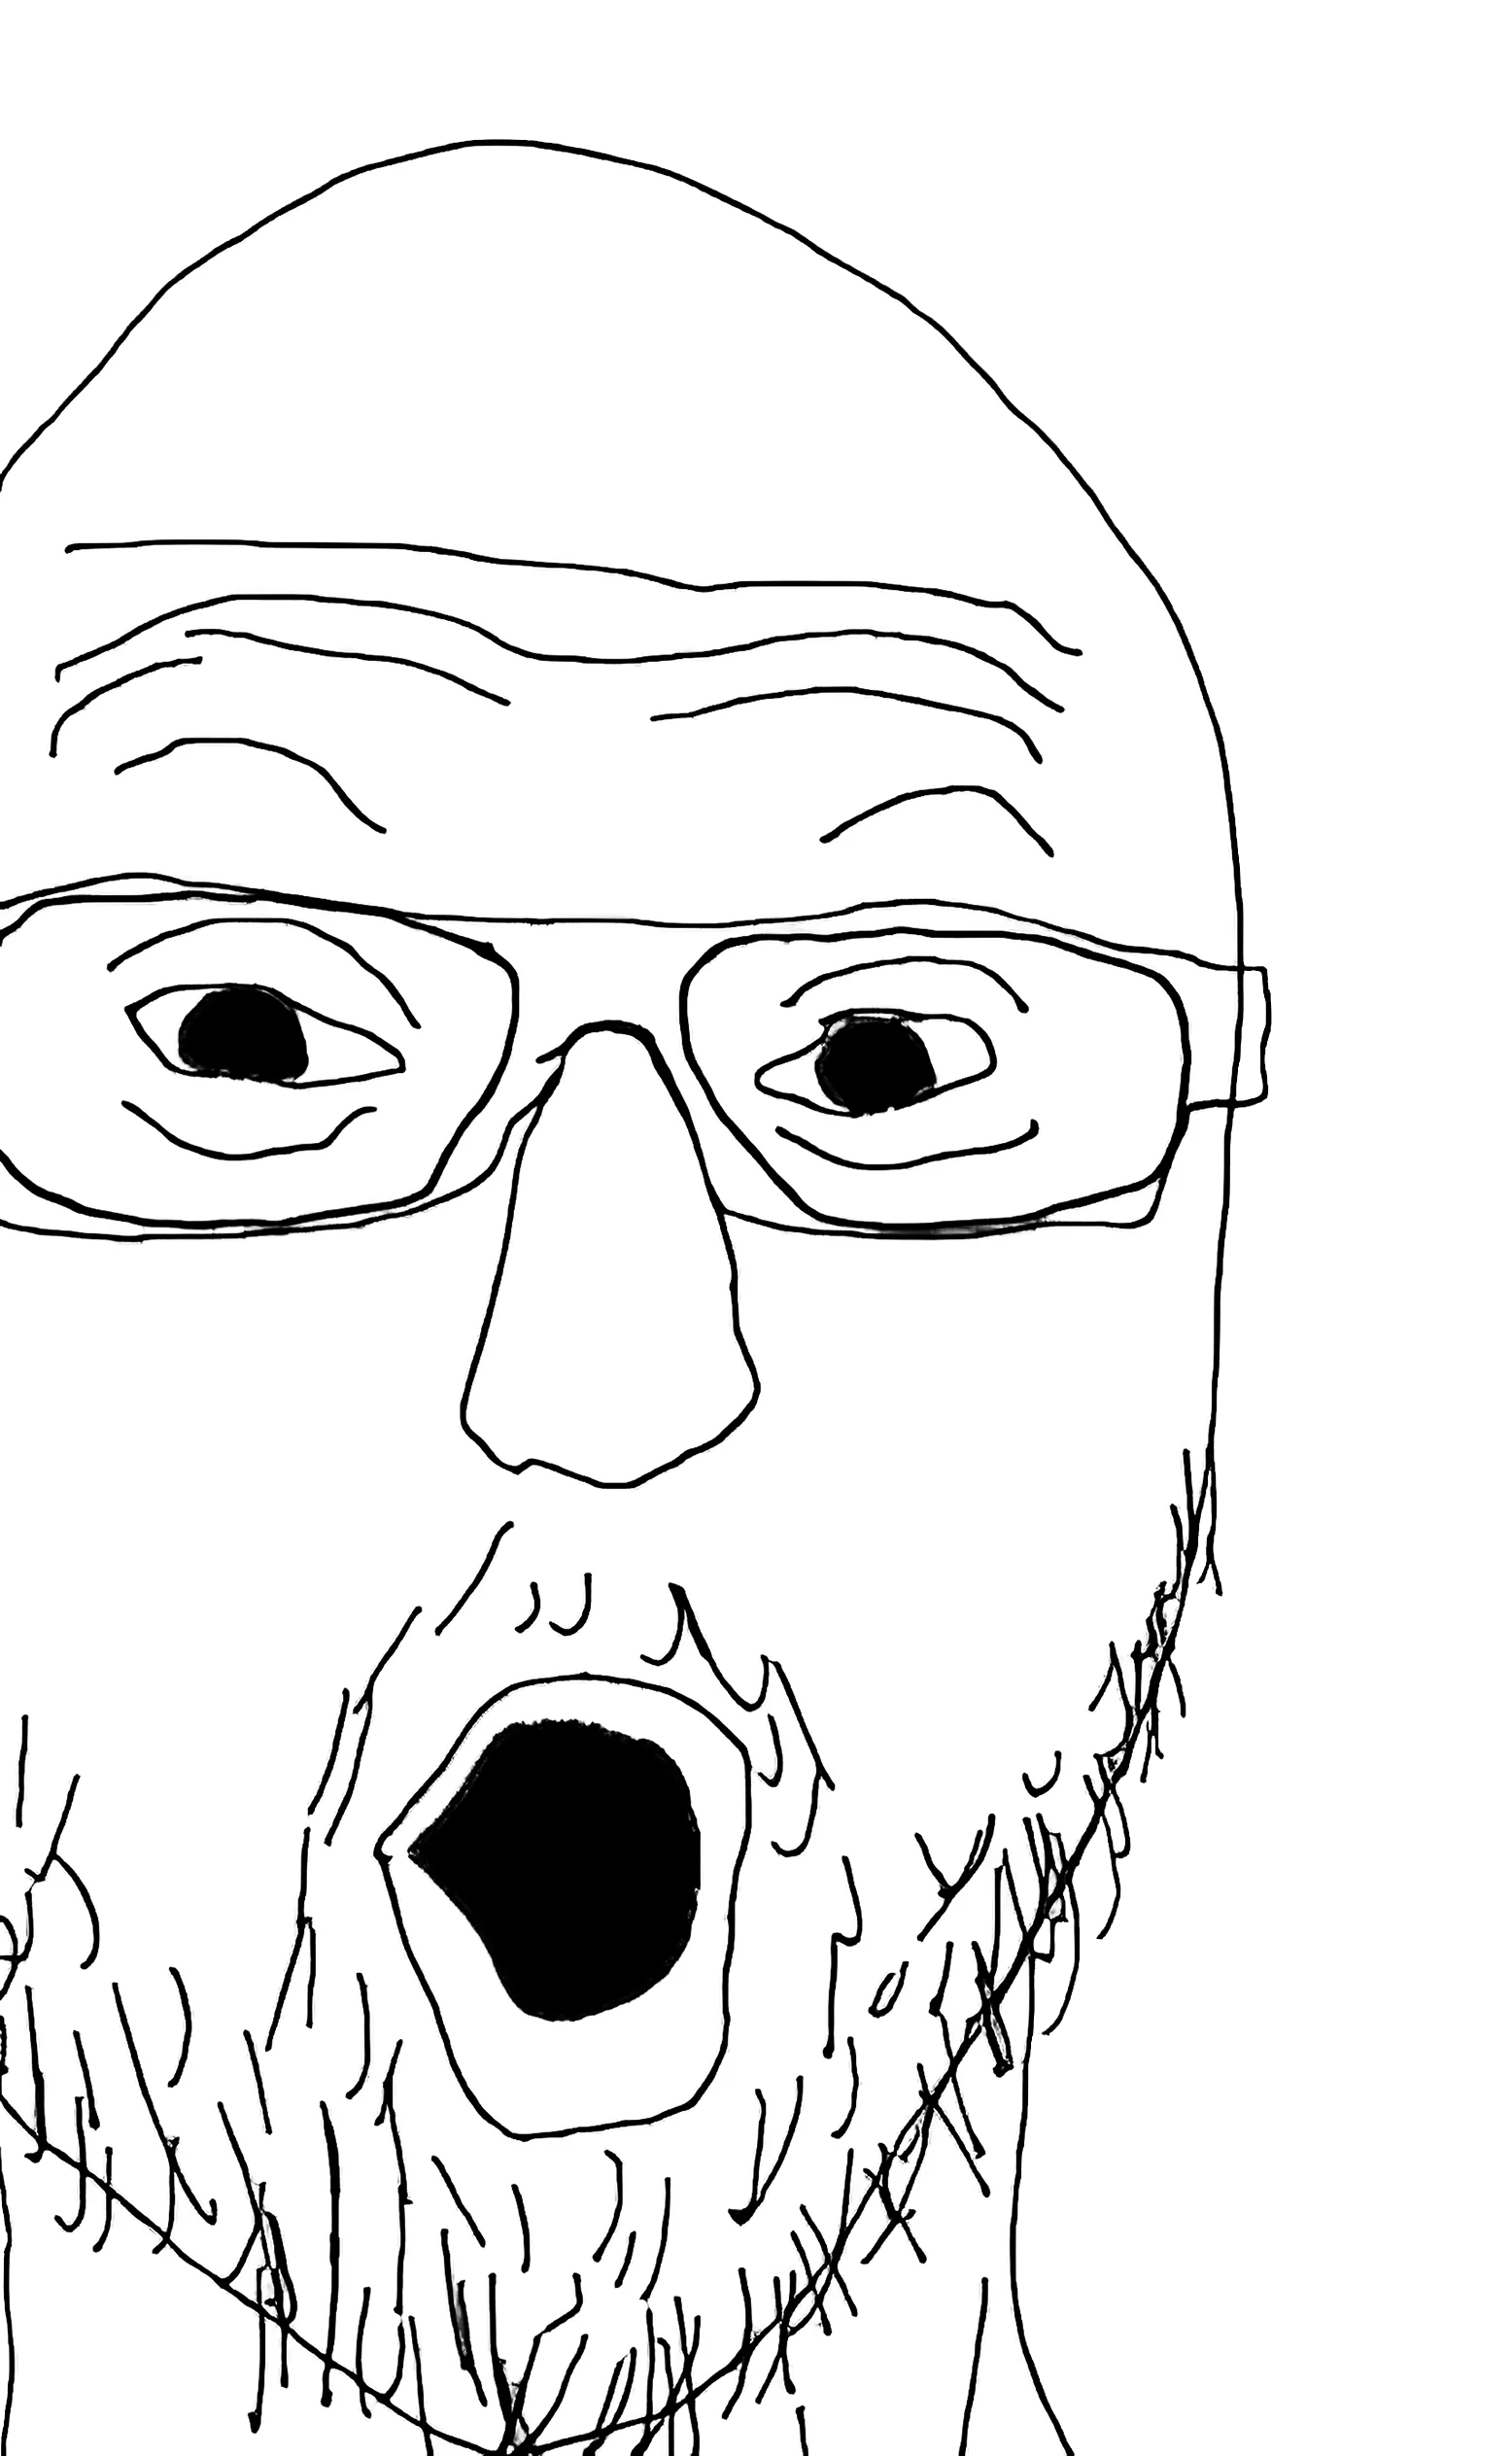
\includegraphics[height=6.15cm]{images/meme_oliva_left.png}};
  \node[anchor=south east,inner sep=0pt]
    at ([xshift=.08cm,yshift=-.14cm]current page.south east)
    {
\includegraphics[height=5.72cm]{images/meme_oliva_right.png}};

  % Paper al centro. La propia imagen contiene únicamente el recuadro rojo
  % alrededor del nombre de Julio Oliva.
  \node[rotate=-1.0,draw=white!75,line width=.55pt,inner sep=3pt,
        fill=white,drop shadow={shadow xshift=1.5pt,shadow yshift=-1.5pt,opacity=.45}]
    at ([yshift=-.15cm]current page.center)
    {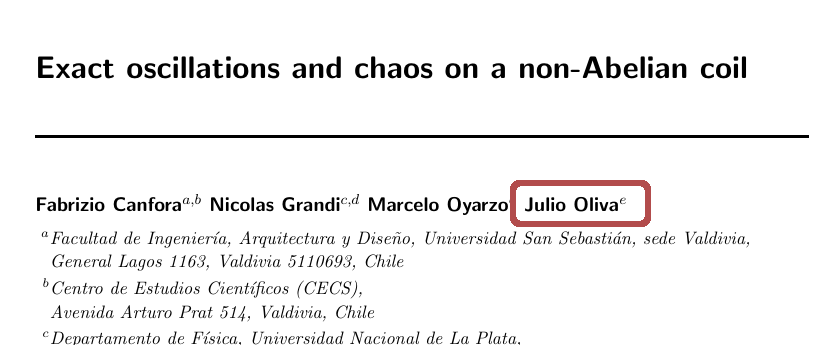
\includegraphics[width=9.15cm,height=4.05cm,keepaspectratio]{images/papers/canfora_oliva_julio_highlight.png}};
\end{tikzpicture}
\end{frame}
}

% --------------------------------------------------
% 13. Lagrangiana SM
% --------------------------------------------------
\begin{frame}{La densidad lagrangiana del Modelo Estándar es el punto de partida}
\vspace{-0.06cm}
\begin{center}
\setlength{\fboxsep}{8pt}
\fcolorbox{UdeCBlue!35}{SoftGray}{%
\begin{minipage}{.94\linewidth}
\small
\begin{align*}
\Lag_{\rm SM}={}&
\textcolor{ChaosRed}{-\frac14G^A_{\mu\nu}G^{A\mu\nu}}
+\textcolor{UdeCBlue}{\left(-\frac14W^a_{\mu\nu}W^{a\mu\nu}-\frac14B_{\mu\nu}B^{\mu\nu}\right)}\\[-1mm]
&+\textcolor{RegularGreen}{\sum_\psi\bar\psi\,\ii\gamma^\mu D_\mu\psi}
+\textcolor{WarmGold}{(D_\mu H)^\dagger D^\mu H-V(H)}
-\textcolor{black!70}{\Lag_Y}.
\end{align*}
\end{minipage}}
\end{center}
\vspace{0.04cm}
\begin{columns}[T,totalwidth=.96\textwidth]
\begin{column}{.22\textwidth}
\centering\textcolor{ChaosRed}{\bfseries $\SU(3)_C$}\par
{\scriptsize gluones y color}
\end{column}
\begin{column}{.26\textwidth}
\centering\textcolor{UdeCBlue}{\bfseries $\SU(2)_L\times\U(1)_Y$}\par
{\scriptsize campos gauge electrodébiles}
\end{column}
\begin{column}{.23\textwidth}
\centering\textcolor{RegularGreen}{\bfseries fermiones}\par
{\scriptsize quarks y leptones}
\end{column}
\begin{column}{.23\textwidth}
\centering\textcolor{WarmGold}{\bfseries Higgs + Yukawa}\par
{\scriptsize vacío, acoplamientos y masas}
\end{column}
\end{columns}
\vspace{0.24cm}
\goldbox{\small Ahora no voy a cuantizarla: voy a apagar sectores de forma explícita hasta obtener un sistema clásico de pocos grados de libertad.}
\sourcebar{Convenciones y estructura: Particle Data Group, Review of Particle Physics.}
\end{frame}

% --------------------------------------------------
% 14. Apagado 1
% --------------------------------------------------
\begin{frame}{Apagado 1: $\psi=0$ elimina explícitamente fermiones y Yukawa}
\small
\[
\Lag_{\rm SM}=\Lag_{\rm gauge}+\underbrace{\sum_\psi\bar\psi\,\ii\gamma^\mu D_\mu\psi}_{\Lag_{\rm ferm}}
+(D_\mu H)^\dagger D^\mu H-V(H)-\Lag_Y.
\]
\[
\psi=0
\quad\Longrightarrow\quad
\bar\psi\,\ii\gamma^\mu D_\mu\psi=0,
\qquad
\Lag_Y\sim \bar\psi H\psi=0.
\]
\[
\boxed{
\Lag_{\rm bos}=
-\frac14G^A_{\mu\nu}G^{A\mu\nu}
-\frac14W^a_{\mu\nu}W^{a\mu\nu}
-\frac14B_{\mu\nu}B^{\mu\nu}
+(D_\mu H)^\dagger D^\mu H-V(H)}
\]
\vspace{0.06cm}
\softbox{\scriptsize Quedan los tres campos gauge y el Higgs; desaparecen materia fermiónica, corrientes fermiónicas y acoplamientos de Yukawa.}
\end{frame}

% --------------------------------------------------
% 15. Apagado 2
% --------------------------------------------------
\begin{frame}{Apagado 2: $G^A_\mu=0$ elimina el sector de color}
\small
\[
G^A_{\mu\nu}
=\partial_\mu G^A_\nu-\partial_\nu G^A_\mu
+g_s f^{ABC}G^B_\mu G^C_\nu.
\]
\[
G^A_\mu=0
\quad\Longrightarrow\quad
G^A_{\mu\nu}=0.
\]
Como ya pusimos $\psi=0$ y el Higgs es singlete de color,
\[
J_C^{A\nu}=0,
\qquad
(D_\mu G^{\mu\nu})^A=J_C^{A\nu}=0,
\]
de modo que el campo de gluones nulo satisface su ecuación de movimiento. Entonces
\[
\boxed{
\Lag_{\rm EW,bos}=
-\frac14W^a_{\mu\nu}W^{a\mu\nu}
-\frac14B_{\mu\nu}B^{\mu\nu}
+(D_\mu H)^\dagger D^\mu H-V(H)}.
\]
\end{frame}

% --------------------------------------------------
% 16. Apagado 3
% --------------------------------------------------
\begin{frame}{Apagado 3: el límite $g'\to0$ desacopla la hipercarga}
\small
\[
D_\mu H=
\left(\partial_\mu-\ii g\frac{\tau^a}{2}W^a_\mu-\ii g'Y_HB_\mu\right)H,
\qquad Y_H=\frac12.
\]
Tomando el límite de parámetros,
\[
\lim_{g'\to0}D_\mu H
=\left(\partial_\mu-\ii g\frac{\tau^a}{2}W^a_\mu\right)H
\equiv D^{(W)}_\mu H.
\]
Por tanto,
\[
\boxed{
\lim_{g'\to0}\Lag_{\rm EW,bos}
=-\frac14W^a_{\mu\nu}W^{a\mu\nu}
-\frac14B_{\mu\nu}B^{\mu\nu}
+(D^{(W)}_\mu H)^\dagger D^{(W)\mu}H-V(H)}.
\]
\softbox{\scriptsize $B_\mu$ todavía existe, pero ya es un campo abeliano libre: dejó de acoplarse al Higgs. Este límite no usa el valor físico de $g'$.}
\end{frame}

% --------------------------------------------------
% 17. Apagado 4
% --------------------------------------------------
\begin{frame}{Apagado 4: una vez desacoplado, elegimos la solución $B_\mu=0$}
\small
Para el campo abeliano libre,
\[
B_{\mu\nu}=\partial_\mu B_\nu-\partial_\nu B_\mu,
\qquad
\partial_\mu B^{\mu\nu}=0.
\]
La elección
\[
B_\mu=0
\quad\Longrightarrow\quad
B_{\mu\nu}=0
\]
satisface esa ecuación. Sustituyendo,
\[
\boxed{
\Lag_{2H}=
-\frac14W^a_{\mu\nu}W^{a\mu\nu}
+(D^{(W)}_\mu H)^\dagger D^{(W)\mu}H-V(H)}.
\]
con
\[
W^a_{\mu\nu}=\partial_\mu W^a_\nu-\partial_\nu W^a_\mu
+g\epsilon^{abc}W^b_\mu W^c_\nu.
\]
\goldbox{\scriptsize El término $g\epsilon^{abc}W^b_\mu W^c_\nu$ mantiene la auto-interacción no abeliana que luego producirá el acoplamiento cuártico.}
\end{frame}

% --------------------------------------------------
% 18. Resumen apagados
% --------------------------------------------------
\begin{frame}{Los cuatro apagados dejan una teoría $\SU(2)$--Higgs}
\begin{columns}[T,totalwidth=.96\textwidth]
\begin{column}{.51\textwidth}
\small
\[
\boxed{\Lag_{2H}= -\frac14W^a_{\mu\nu}W^{a\mu\nu}+(D_\mu H)^\dagger D^\mu H-V(H)}
\]
\[
W^a_{\mu\nu}=\partial_\mu W^a_\nu-\partial_\nu W^a_\mu+g\epsilon^{abc}W^b_\mu W^c_\nu.
\]
\goldbox{\scriptsize Aún es una teoría de campos: depende de $\mathbf x$ y $t$ y conserva infinitos grados de libertad.}
\end{column}
\begin{column}{.42\textwidth}
\begin{tikzpicture}[>=Latex,node distance=.29cm]
\node[draw=UdeCBlue,rounded corners=3pt,fill=SoftBlue,text width=4.2cm,align=center] (sm) {$\Lag_{\rm SM}$};
\node[draw=UdeCBlue,rounded corners=3pt,fill=white,text width=4.2cm,align=center,below=of sm] (f) {$\psi=0$};
\node[draw=UdeCBlue,rounded corners=3pt,fill=white,text width=4.2cm,align=center,below=of f] (c) {$G^A_\mu=0$};
\node[draw=WarmGold,rounded corners=3pt,fill=SoftGold,text width=4.2cm,align=center,below=of c] (gp) {$g'\to0$};
\node[draw=WarmGold,rounded corners=3pt,fill=SoftGold,text width=4.2cm,align=center,below=of gp] (b) {$B_\mu=0$};
\node[draw=ChaosRed,rounded corners=3pt,fill=ChaosRed!6,text width=4.2cm,align=center,below=of b] (l) {$\Lag_{2H}$};
\draw[->,thick] (sm)--(f);\draw[->,thick] (f)--(c);\draw[->,thick] (c)--(gp);\draw[->,thick] (gp)--(b);\draw[->,thick] (b)--(l);
\end{tikzpicture}
\end{column}
\end{columns}
\end{frame}

% --------------------------------------------------
% 19. Homogeneidad: densidad -> lagrangiano mecánico
% --------------------------------------------------
\begin{frame}{Homogeneidad: de una densidad lagrangiana a un lagrangiano mecánico}
\small
Trabajamos en $2+1$ dimensiones, $U=I\times\Omega$, e imponemos
\[
\boxed{\partial_iW^a_\mu=0,\qquad \partial_iH=0,\qquad i=1,2.}
\]
Entonces $\Lag_{2H}$ ya no depende de la posición dentro de $\Omega$:
\[
\begin{aligned}
S
&=\int_I\dd t\int_\Omega\dd^2x\,\Lag_{2H}(t)\\
&=|\Omega|\int_I\dd t\,\Lag_{\rm hom}(t)
\equiv\int_I\dd t\,L_{\rm hom}(t).
\end{aligned}
\]
Por definición,
\[
\boxed{L_{\rm hom}(t)=|\Omega|\,\Lag_{\rm hom}(t).}
\]
Trabajando por unidad de área, $|\Omega|=1$,
\[
\boxed{L_{\rm hom}=\Lag_{\rm hom}.}
\]
\goldbox{\scriptsize Este es el paso que convierte la densidad de la teoría de campos homogénea en el lagrangiano del sistema mecánico reducido.}
\end{frame}

% --------------------------------------------------
% 20. Gauge temporal y componentes de campo
% --------------------------------------------------
\begin{frame}{Gauge temporal: qué componentes del campo sobreviven}
\small
Elegimos
\[
\boxed{W^a_0=0}.
\]
Con homogeneidad espacial,
\[
W^a_{0i}=\partial_0W^a_i-\underbrace{\partial_iW^a_0}_{0}
+g\epsilon^{abc}\underbrace{W^b_0}_{0}W^c_i
=\dot W^a_i,
\]
\[
W^a_{12}=\underbrace{\partial_1W^a_2-\partial_2W^a_1}_{0}
+g\epsilon^{abc}W^b_1W^c_2.
\]
Escribiendo $\vec W_i=(W_i^1,W_i^2,W_i^3)$,
\[
\boxed{\vec E_i=\dot{\vec W}_i,
\qquad
\vec B=\vec W_{12}=g\,\vec W_1\times\vec W_2.}
\]
La ecuación de Gauss permanece como restricción:
\[
\boxed{(D_iE_i)^a=J_H^{a0}.}
\]
\end{frame}

% --------------------------------------------------
% 21. Higgs congelado
% --------------------------------------------------
\begin{frame}{Congelar el Higgs conserva la escala de masa y elimina su dinámica}
\begin{columns}[T,totalwidth=.96\textwidth]
\begin{column}{.54\textwidth}
\small
\[
V(H)=-m^2H^\dagger H+\lambda(H^\dagger H)^2,
\qquad
H_0=\frac1{\sqrt2}\begin{pmatrix}0\\v_{\rm EW}\end{pmatrix}.
\]
Con $\partial_\mu H_0=0$,
\[
D_\mu H_0=-\ii g\frac{\tau^a}{2}W^a_\mu H_0,
\]
\[
(D_\mu H_0)^\dagger D^\mu H_0
=\frac{g^2v_{\rm EW}^2}{8}W^a_\mu W^{\mu a}.
\]
\[
M_W^2=\frac{g^2v_{\rm EW}^2}{4}.
\]
\end{column}
\begin{column}{.38\textwidth}
\softbox{\small \textbf{Conservo:} la escala $v_{\rm EW}$ y el término de masa gauge.}
\vspace{0.09cm}
\goldbox{\small \textbf{Elimino:} fluctuación radial del Higgs, Goldstones y retroacción dinámica gauge--Higgs.}
\vspace{0.09cm}
{\scriptsize Es una aproximación de fondo rígido, no una truncación exacta general.}
\end{column}
\end{columns}
\end{frame}

% --------------------------------------------------
% 22. Derivación explícita Lhom
% --------------------------------------------------
\begin{frame}{Ahora sí aparece $L_{\rm hom}$: sustitución término a término}
\small
Con signatura $(+,-,-)$,
\[
-\frac14W^a_{\mu\nu}W^{a\mu\nu}
=\frac12\left(\|\dot{\vec W}_1\|^2+\|\dot{\vec W}_2\|^2\right)
-\frac12\|\vec W_{12}\|^2,
\]
y como $\vec W_{12}=g\vec W_1\times\vec W_2$,
\[
-\frac14W^2
=\frac12\sum_{i=1}^2\|\dot{\vec W}_i\|^2
-\frac{g^2}{2}\|\vec W_1\times\vec W_2\|^2.
\]
Además, con $W_0=0$,
\[
(D_\mu H_0)^\dagger D^\mu H_0
=-\frac{g^2v_{\rm EW}^2}{8}\sum_{i=1}^2\|\vec W_i\|^2.
\]
Quitando la constante $V(H_0)$ y usando $|\Omega|=1$,
\[
\boxed{L_{\rm hom}
=\frac12\sum_i\|\dot{\vec W}_i\|^2
-\frac{g^2}{2}\|\vec W_1\times\vec W_2\|^2
-\frac{g^2v_{\rm EW}^2}{8}\sum_i\|\vec W_i\|^2.}
\]
\end{frame}

% --------------------------------------------------
% 23. Ansatz
% --------------------------------------------------
\begin{frame}{El ansatz conserva dos amplitudes y la interacción no abeliana}
\begin{columns}[T,totalwidth=.97\textwidth]
\begin{column}{.48\textwidth}
\small
\[
\boxed{\vec W_1=q_1(t)\vec e_1,
\qquad
\vec W_2=q_2(t)\vec e_2.}
\]
Entonces
\[
\|\dot{\vec W}_1\|^2+\|\dot{\vec W}_2\|^2
=\dot q_1^2+\dot q_2^2,
\]
\[
\|\vec W_1\times\vec W_2\|^2=q_1^2q_2^2,
\qquad
\|\vec W_1\|^2+\|\vec W_2\|^2=q_1^2+q_2^2.
\]
\end{column}
\begin{column}{.45\textwidth}
\small
La restricción de Gauss se satisface:
\[
\sum_i\vec W_i\times\dot{\vec W}_i
=q_1\dot q_1\,\vec e_1\times\vec e_1
+q_2\dot q_2\,\vec e_2\times\vec e_2=0.
\]
Por tanto,
\[
\boxed{L_{\rm red}=\frac12(\dot q_1^2+\dot q_2^2)
-\frac{g^2v_{\rm EW}^2}{8}(q_1^2+q_2^2)
-\frac{g^2}{2}q_1^2q_2^2.}
\]
\end{column}
\end{columns}
\end{frame}

% --------------------------------------------------
% 24. Hamiltoniano e interpretación
% --------------------------------------------------
\begin{frame}{La transformación de Legendre revela el Hamiltoniano no lineal}
\begin{columns}[T,totalwidth=.97\textwidth]
\begin{column}{.50\textwidth}
\small
\[
p_i=\frac{\partial L_{\rm red}}{\partial\dot q_i}=\dot q_i,
\qquad
H=p_i\dot q_i-L_{\rm red}.
\]
\[
\boxed{H_{\rm red}=\frac12(p_1^2+p_2^2)
+\frac{g^2v_{\rm EW}^2}{8}(q_1^2+q_2^2)
+\frac{g^2}{2}q_1^2q_2^2.}
\]
\end{column}
\begin{column}{.43\textwidth}
\begin{tikzpicture}[node distance=.27cm]
\node[draw=UdeCBlue,rounded corners=3pt,fill=SoftBlue,text width=4.2cm,align=center] (k) {$\frac12(p_1^2+p_2^2)$\\\scriptsize energía cinética de los modos};
\node[draw=RegularGreen,rounded corners=3pt,fill=RegularGreen!7,text width=4.2cm,align=center,below=of k] (m) {$\frac{g^2v_{\rm EW}^2}{8}(q_1^2+q_2^2)$\\\scriptsize masa gauge inducida por el vacío};
\node[draw=WarmGold,rounded corners=3pt,fill=SoftGold,text width=4.2cm,align=center,below=of m] (c) {$\frac{g^2}{2}q_1^2q_2^2$\\\scriptsize acoplamiento no abeliano};
\end{tikzpicture}
\vspace{0.08cm}
{\scriptsize Cerca del origen domina el término cuadrático; a mayor amplitud el término cuártico acopla con fuerza los dos modos.}
\end{column}
\end{columns}
\end{frame}

% --------------------------------------------------
% 25. Poincaré
% --------------------------------------------------
\begin{frame}{La sección de Poincaré vuelve visible la estructura de las órbitas}
\begin{columns}[T,totalwidth=.98\textwidth]
\begin{column}{.66\textwidth}
\centering
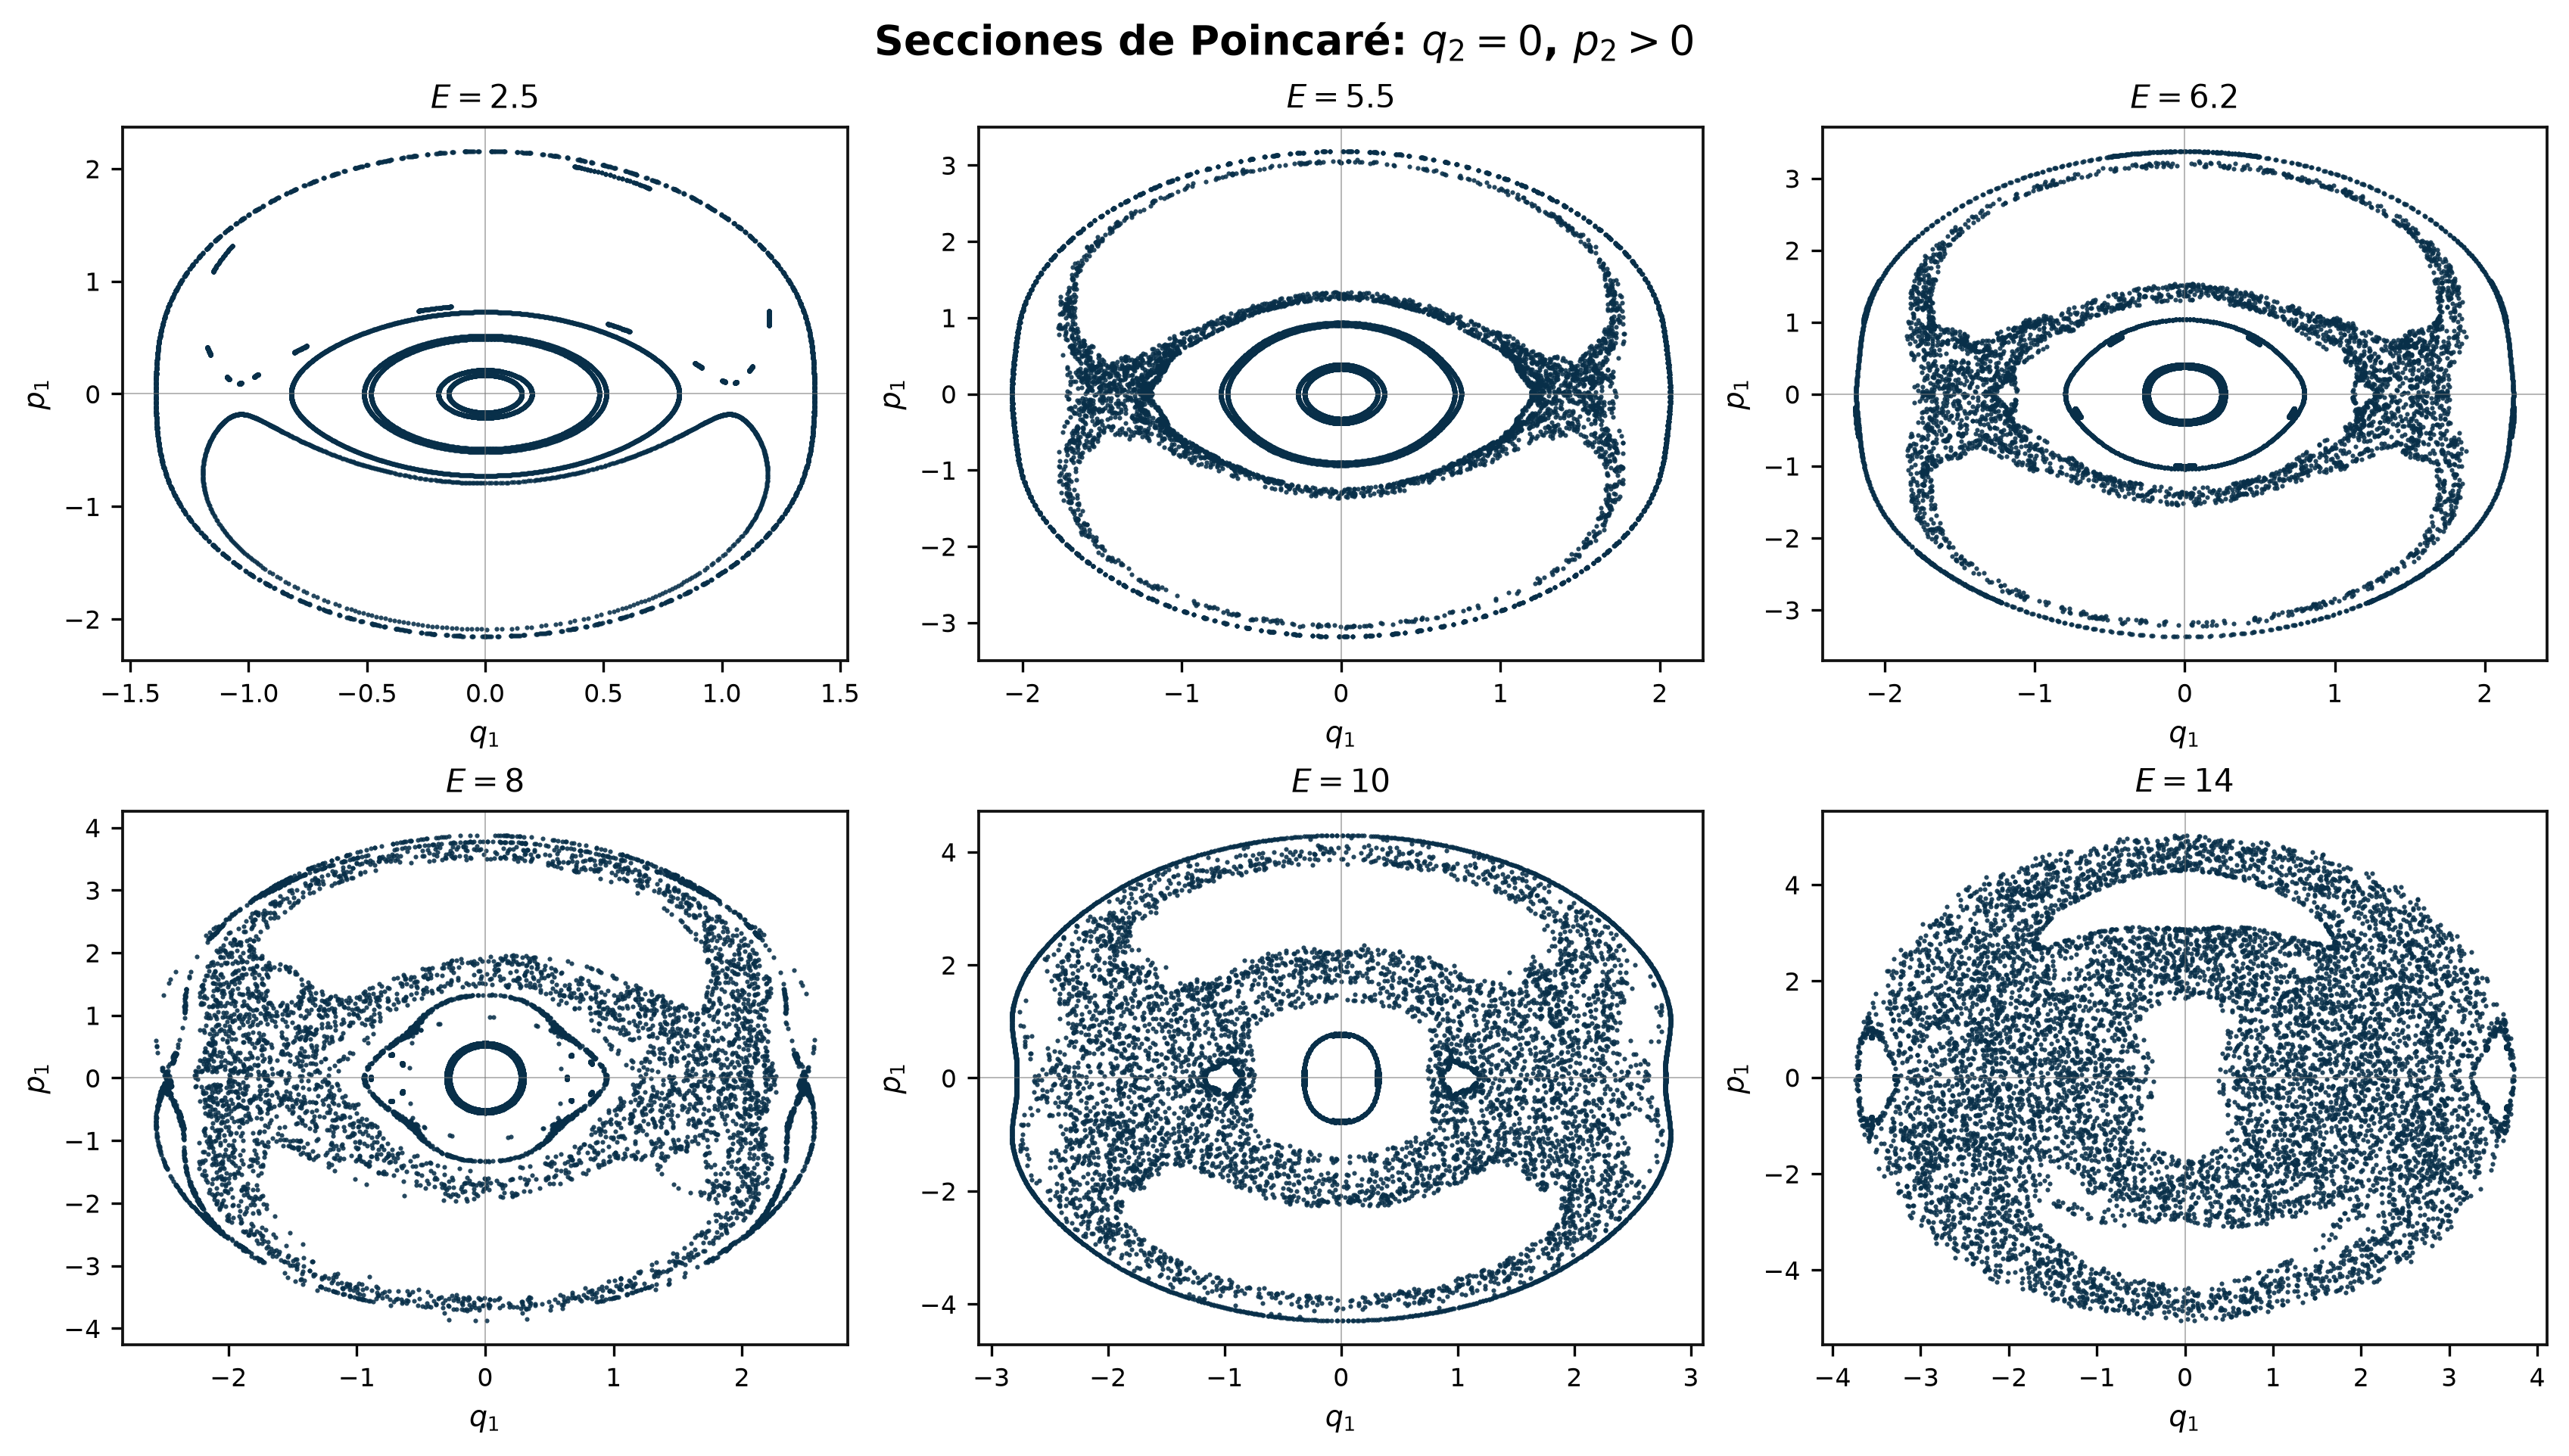
\includegraphics[width=\linewidth,height=5.55cm,keepaspectratio]{images/figures/salasnich_poincare_6E_contraste.png}
\end{column}
\begin{column}{.30\textwidth}
\small
El espacio de fases es
\[
(q_1,q_2,p_1,p_2)\in\mathbb R^4.
\]
A energía fija $H=E$, registramos cada cruce con
\[
\boxed{q_2=0,\qquad p_2>0}
\]
y dibujamos $(q_1,p_1)$.
\vspace{0.06cm}
\begin{itemize}\small\setlength\itemsep{.15cm}
\item curvas/islas: regularidad;
\item regiones rellenas: caos;
\item mezcla de ambas: espacio de fases mixto.
\end{itemize}
\goldbox{\scriptsize Cada panel reúne varias órbitas compatibles con la misma energía para hacer visible la geometría global de la sección.}
\end{column}
\end{columns}
\end{frame}

% --------------------------------------------------
% 26. Otras reducciones
% --------------------------------------------------
\begin{frame}{El método se repite: otras reducciones producen otras secciones}
\begin{columns}[T,totalwidth=.98\textwidth]
\begin{column}{.49\textwidth}
\centering
{\bfseries\color{UdeCBlue}Sector $\SU(2)$--Higgs homogéneo}\par
\vspace{0.05cm}
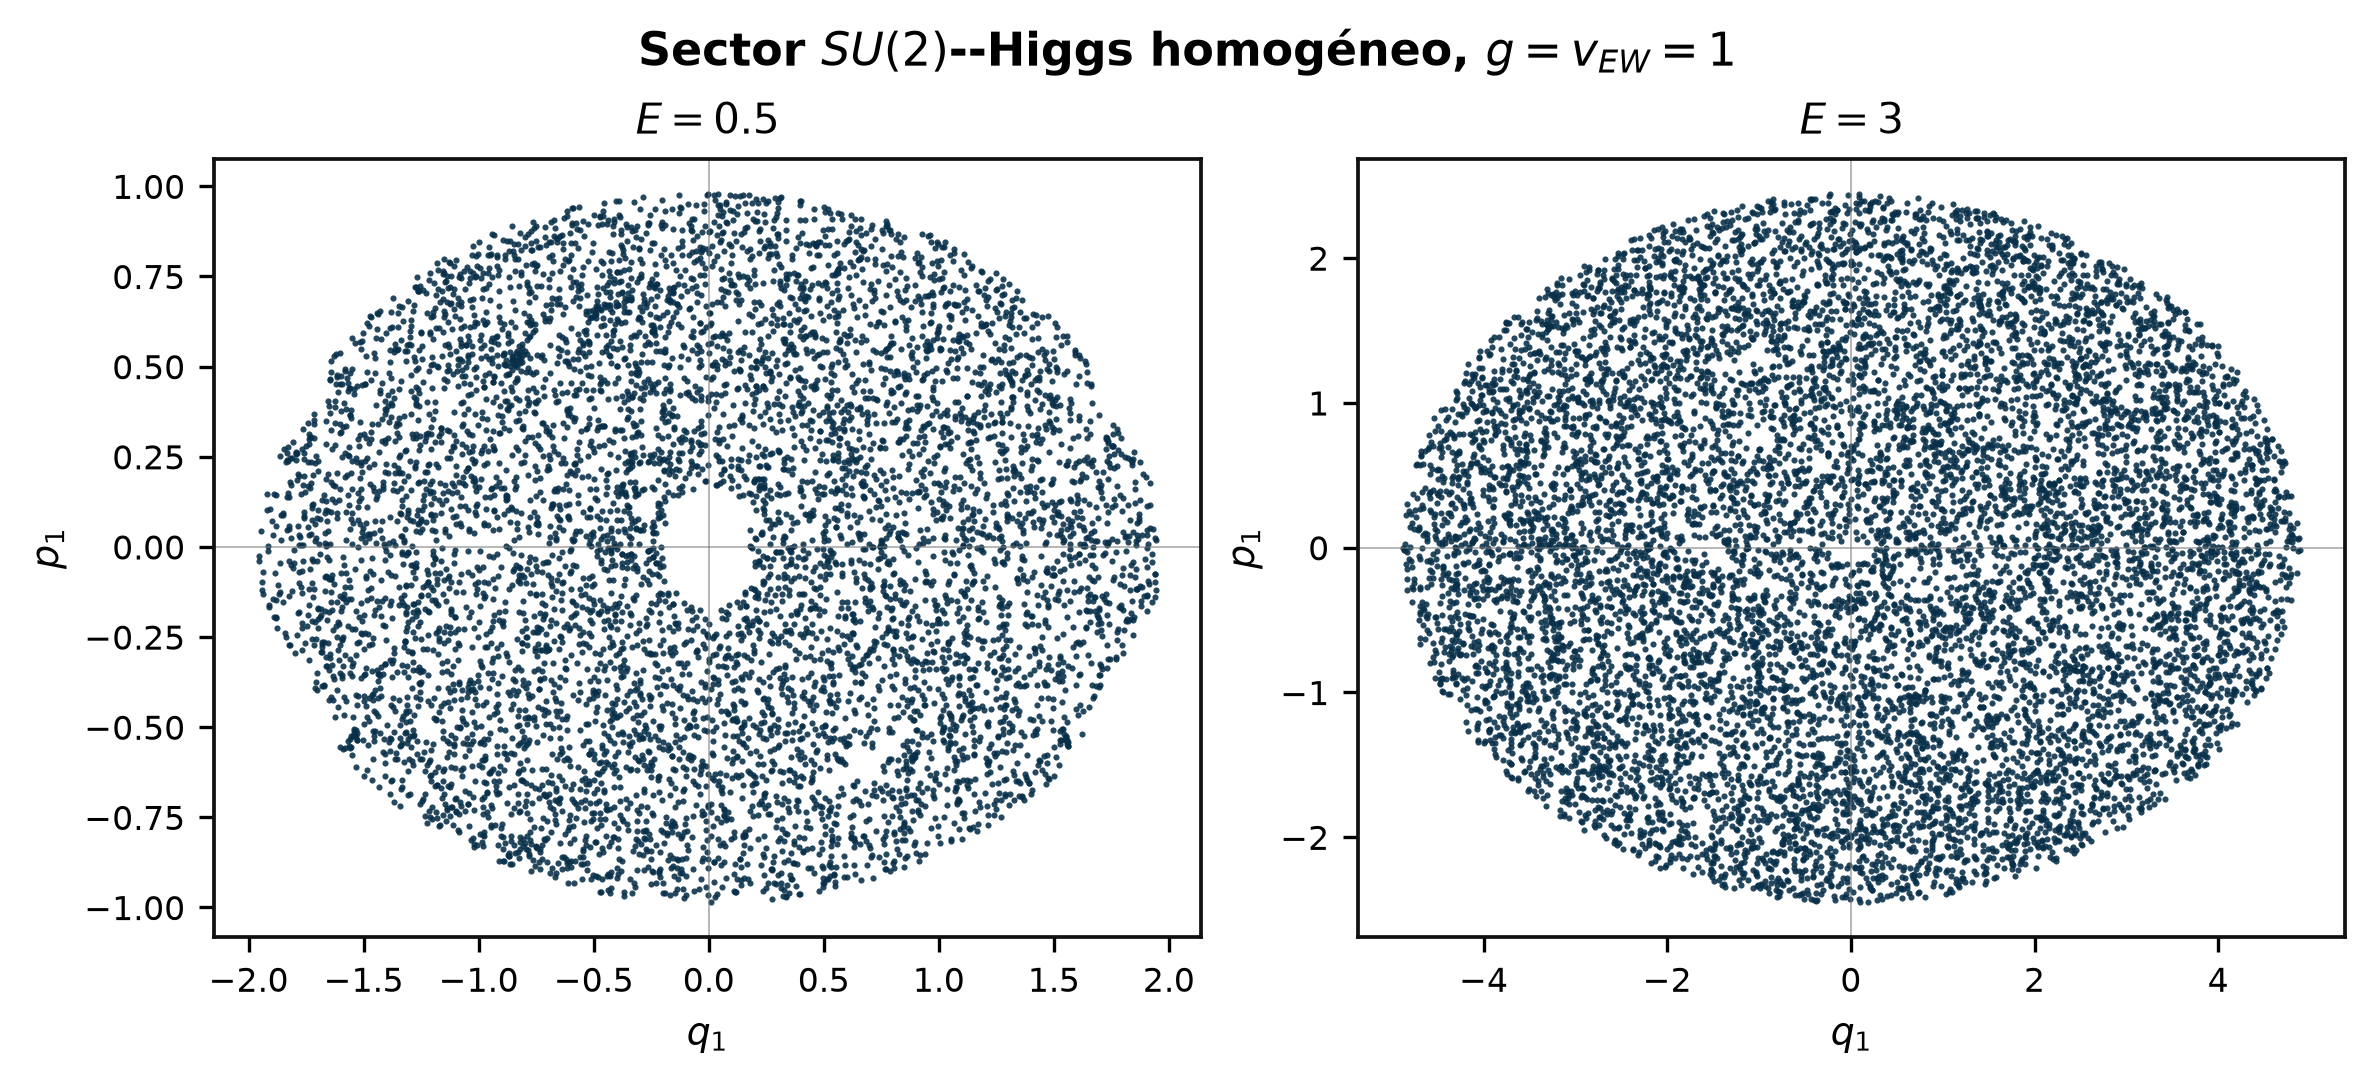
\includegraphics[width=\linewidth,height=4.55cm,keepaspectratio]{images/figures/electroweak_poincare_contraste.png}
{\scriptsize La misma ruta de doblete, aquí con $g=v_{\rm EW}=1$, cambia la escala del término cuadrático y por tanto la geometría del flujo.}
\end{column}
\begin{column}{.49\textwidth}
\centering
{\bfseries\color{WarmGold}Dos diones BPS a baja energía}\par
\vspace{0.05cm}
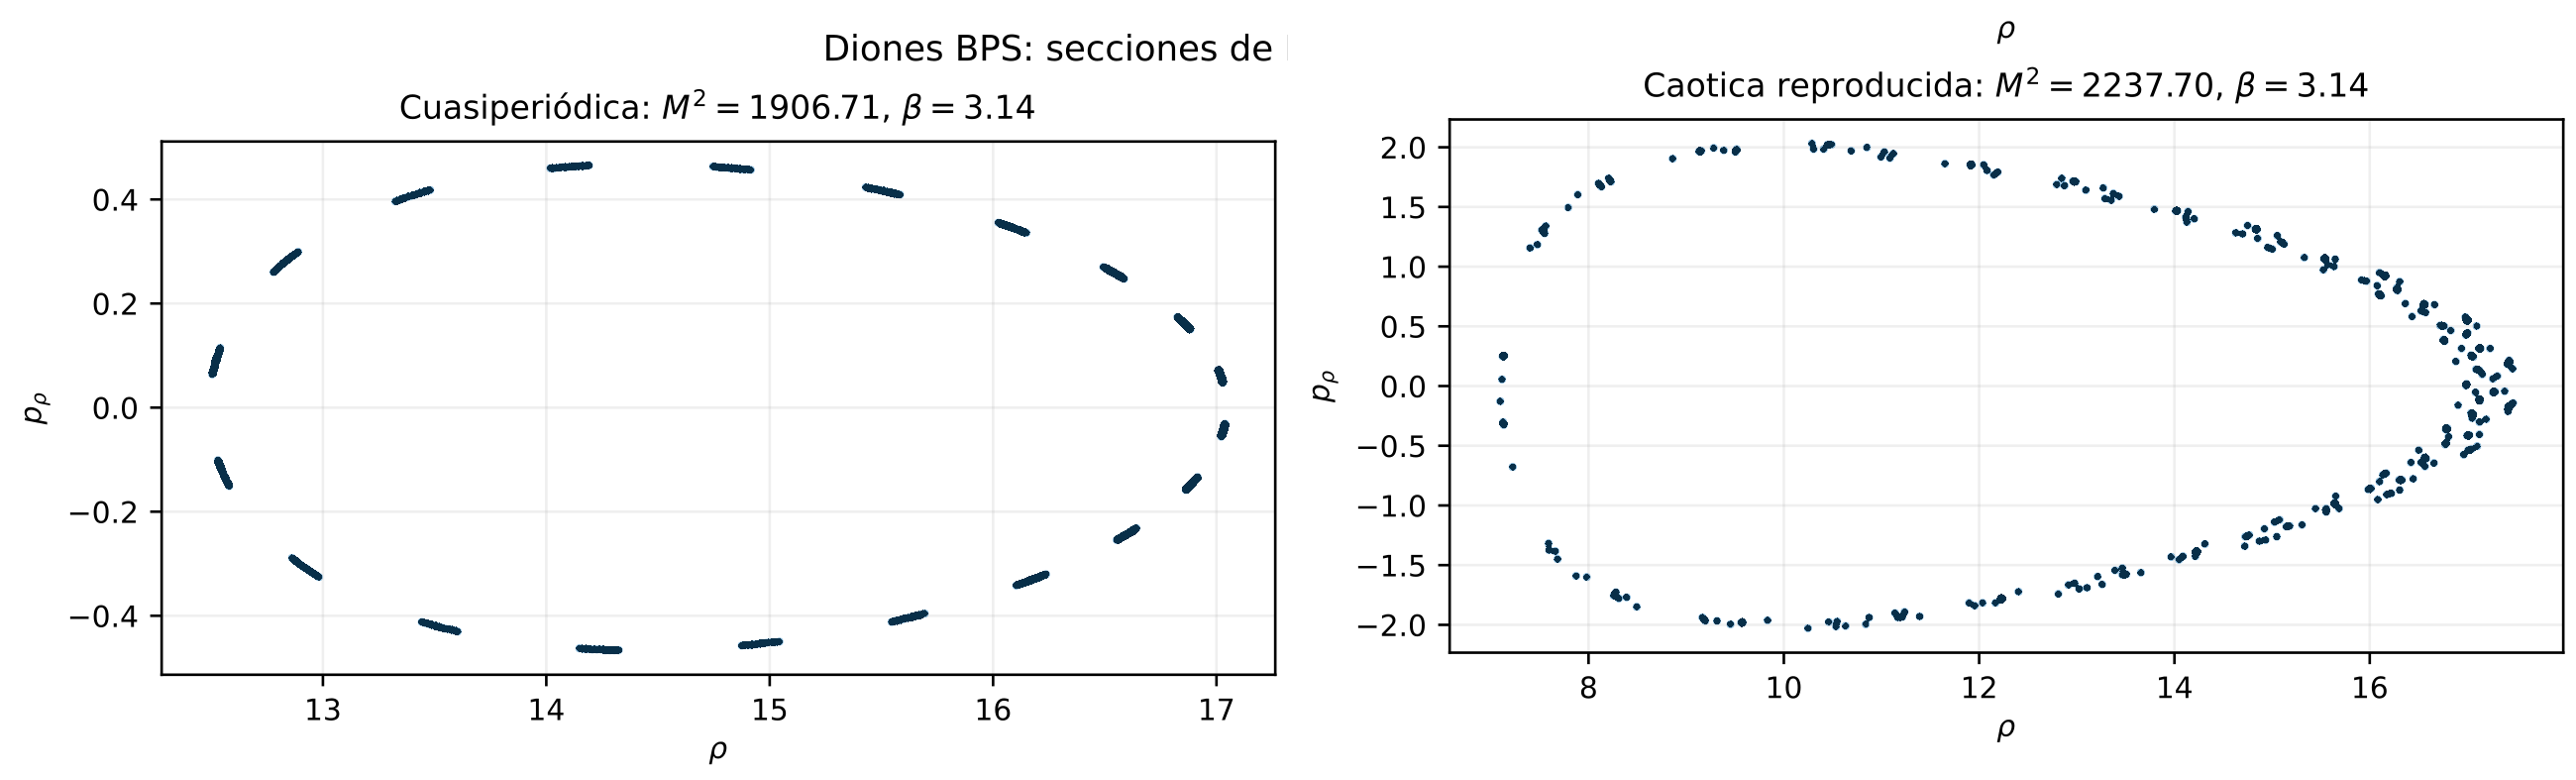
\includegraphics[width=\linewidth,height=4.55cm,keepaspectratio]{images/figures/dyons_poincare_2panel_contraste.png}
{\scriptsize Otra reducción de dinámica $\SU(2)$ Yang--Mills--Higgs: la aproximación geodésica conserva un espacio de fases finito y muestra regiones cuasiperiódicas y caóticas.}
\end{column}
\end{columns}
\sourcebar{Diones BPS: Fariello, Forkel y Krein, Phys. Rev. D 72, 105015 (2005).}
\end{frame}

% --------------------------------------------------
% 27. Canfora / Oliva
% --------------------------------------------------
\begin{frame}{Una reducción en $3+1$: Canfora--Grandi--Oyarzo--Oliva}
\begin{columns}[T,totalwidth=.98\textwidth]
\begin{column}{.63\textwidth}
\centering
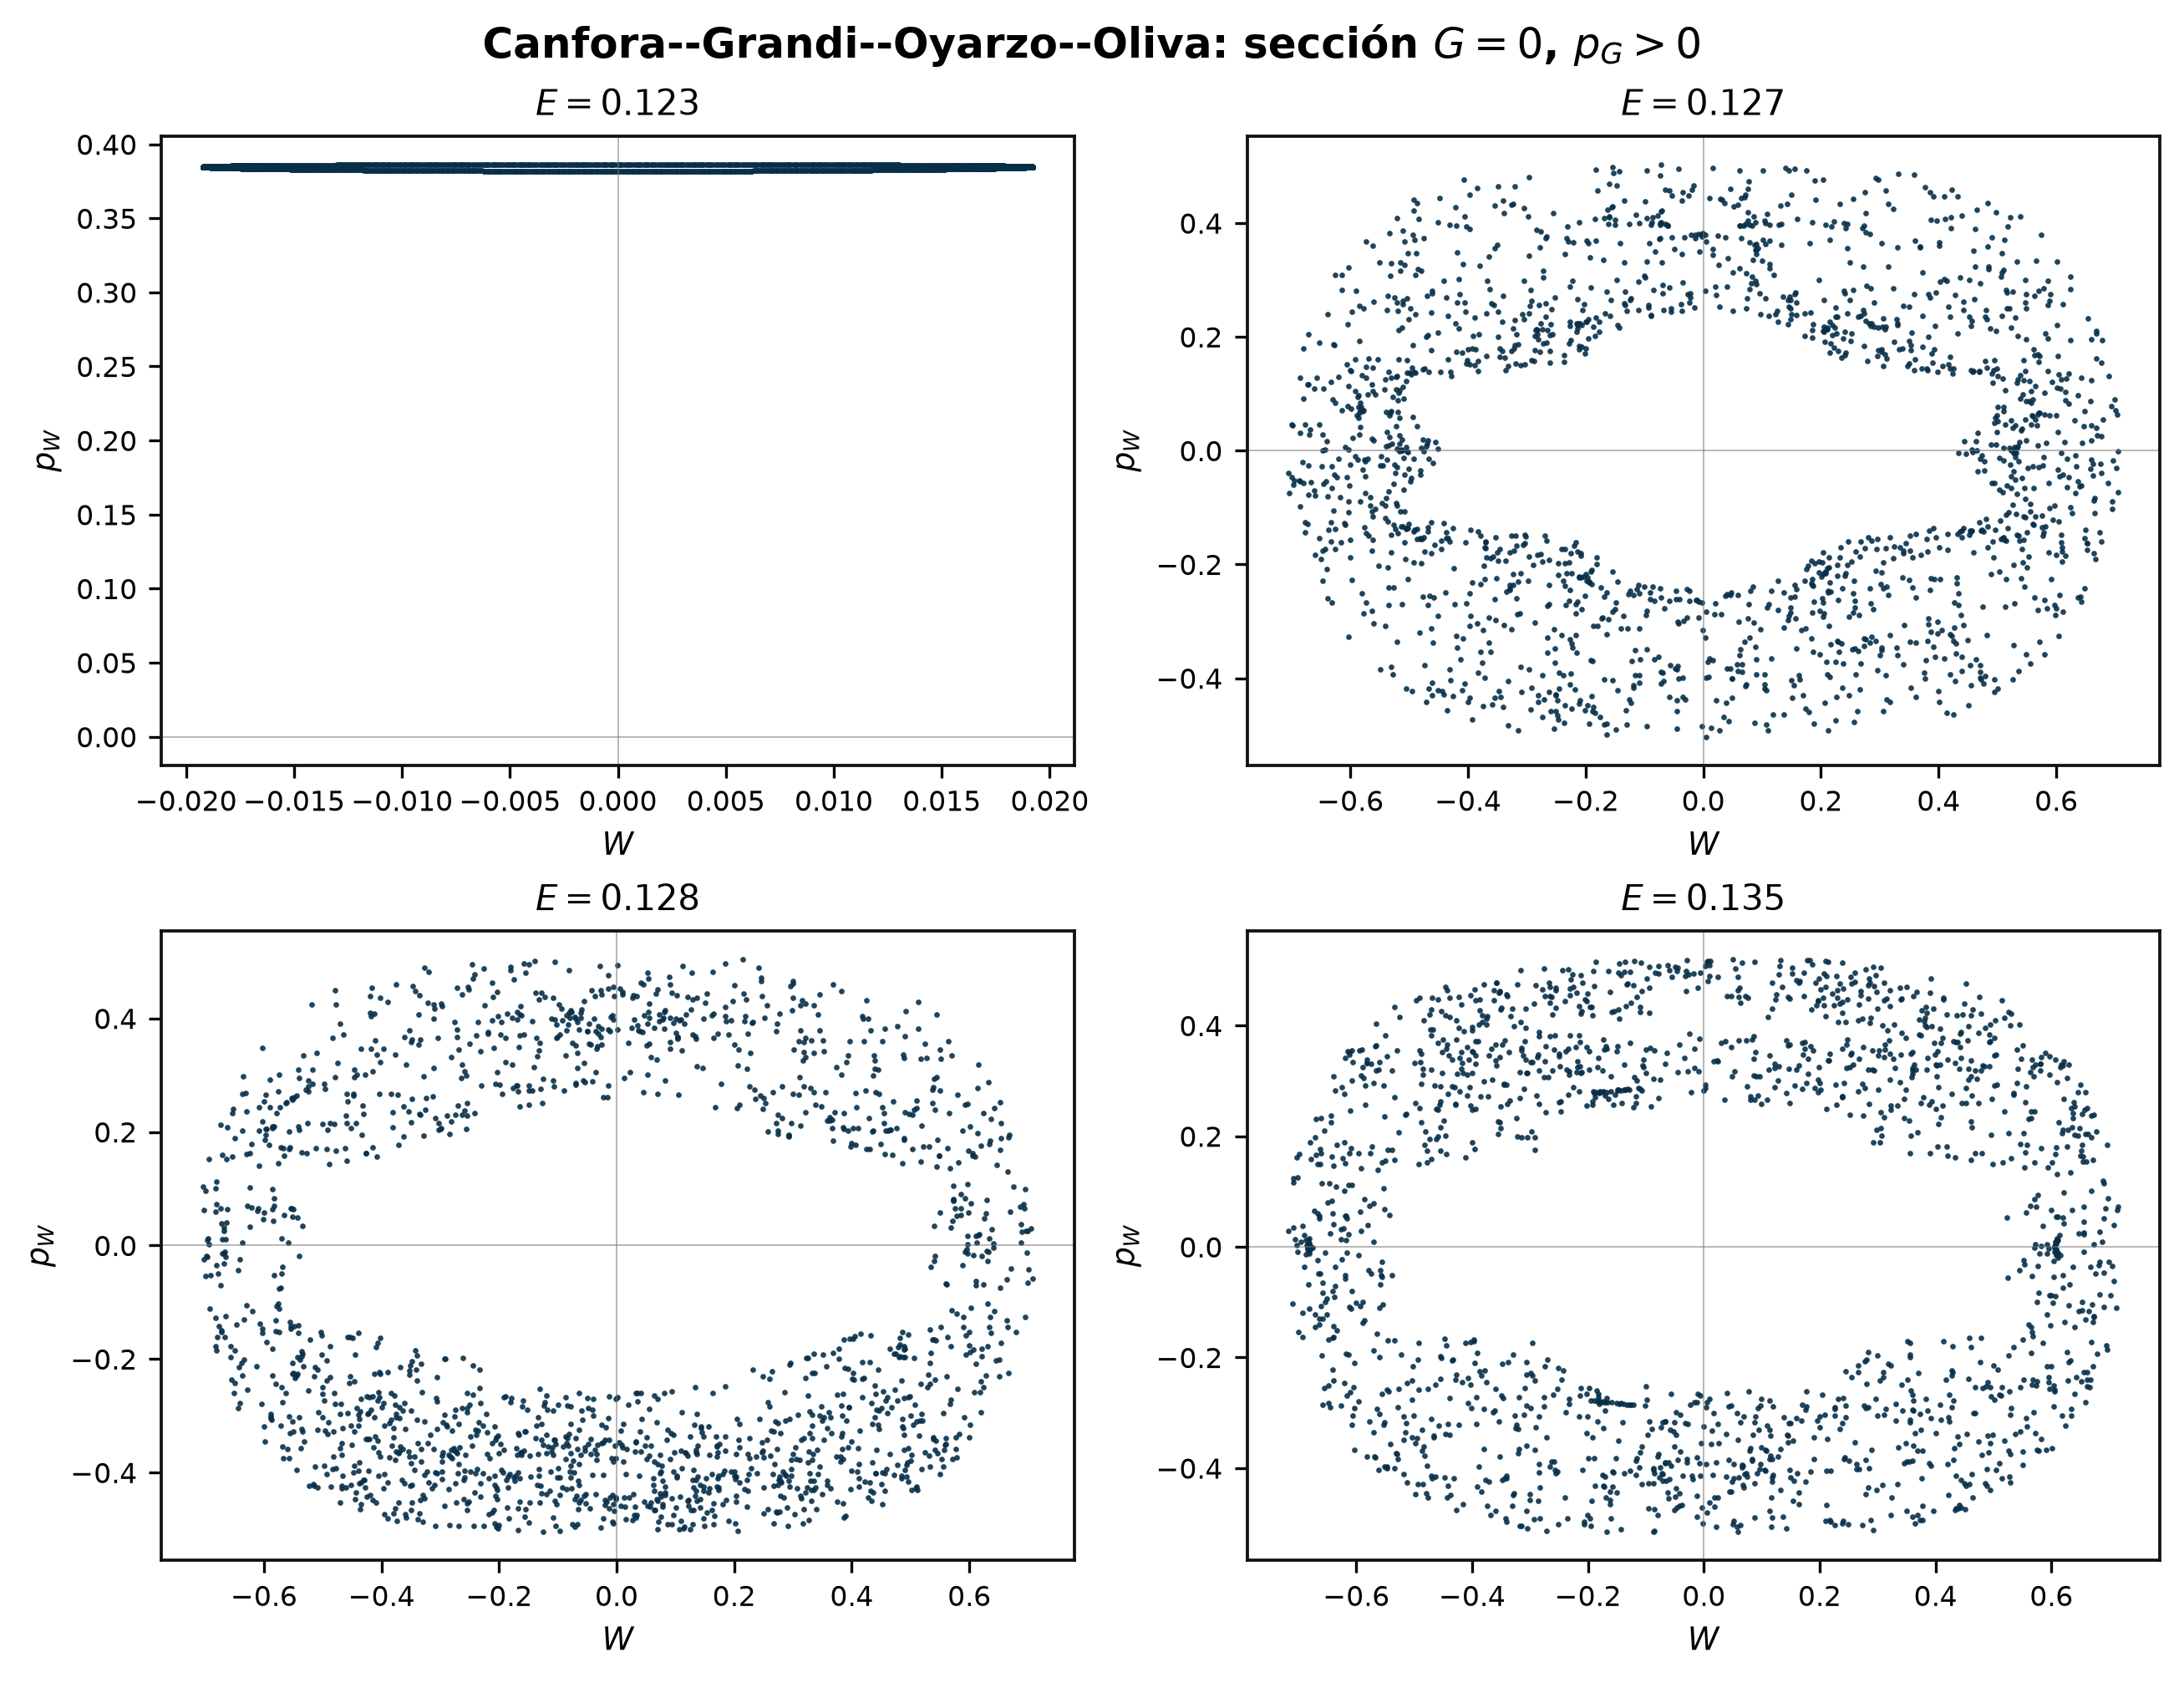
\includegraphics[width=\linewidth,height=5.45cm,keepaspectratio]{images/figures/canfora_poincare_contraste.png}
\end{column}
\begin{column}{.32\textwidth}
\small
El ansatz del modelo de Georgi--Glashow reduce las EDP a
\[
\ddot G+4W^2G+\lambda G(G^2-\nu^2)=0,
\]
\[
\ddot W+4G^2W+2W^3=0.
\]
Aquí se muestra $\nu=0$, $\lambda=1$ y la sección
\[
G=0,\qquad p_G>0,
\]
en el plano $(W,p_W)$.
\vspace{0.08cm}
\goldbox{\scriptsize El artículo reporta una transición alrededor de $E\simeq0.127$--$0.128$ para este régimen; la sección numérica reproduce ese cambio cualitativo.}
\end{column}
\end{columns}
\sourcebar{F. Canfora, N. Grandi, M. Oyarzo y J. Oliva, ``Exact oscillations and chaos on a non-Abelian coil'', Nucl. Phys. B 1004 (2024) 116553.}
\end{frame}

% --------------------------------------------------
% 29. Conclusión
% --------------------------------------------------
\begin{frame}{Conclusión}
\vspace{0.35cm}
\begin{center}
{\Large\bfseries\color{UdeCBlue} ¿Dónde quedó el caos clásico?}
\end{center}
\vspace{0.38cm}

\begin{columns}[T,totalwidth=.94\textwidth]
\begin{column}{.46\textwidth}
\begin{center}
\setlength{\fboxsep}{10pt}
\fcolorbox{ChaosRed!70}{ChaosRed!6}{%
\begin{minipage}[c][1.62cm][c]{.86\linewidth}
\centering
\large\textbf{No} en el Modelo Estándar\\cuántico completo.
\end{minipage}}
\end{center}
\end{column}
\begin{column}{.46\textwidth}
\begin{center}
\setlength{\fboxsep}{10pt}
\fcolorbox{RegularGreen!70}{RegularGreen!6}{%
\begin{minipage}[c][1.62cm][c]{.86\linewidth}
\centering
\large\textbf{Sí} en un sector clásico\\reducido $\SU(2)$--Higgs.
\end{minipage}}
\end{center}
\end{column}
\end{columns}

\vspace{0.40cm}
\begin{center}
\begin{tikzpicture}[>=Latex,node distance=.22cm]
\node[draw=UdeCBlue,rounded corners=3pt,fill=SoftBlue,inner xsep=8pt,inner ysep=7pt] (a) {$\Lag_{\rm SM}$};
\node[draw=WarmGold,rounded corners=3pt,fill=SoftGold,inner xsep=8pt,inner ysep=7pt,right=.28cm of a] (b) {reducir};
\node[draw=UdeCBlue,rounded corners=3pt,fill=SoftBlue,inner xsep=8pt,inner ysep=7pt,right=.28cm of b] (c) {$H_{\rm red}$};
\node[draw=ChaosRed,rounded corners=3pt,fill=ChaosRed!6,inner xsep=8pt,inner ysep=7pt,right=.28cm of c] (d) {órbitas};
\node[draw=RegularGreen,rounded corners=3pt,fill=RegularGreen!6,inner xsep=8pt,inner ysep=7pt,right=.28cm of d] (e) {caos};
\draw[->,thick,UdeCBlue] (a)--(b);
\draw[->,thick,UdeCBlue] (b)--(c);
\draw[->,thick,UdeCBlue] (c)--(d);
\draw[->,thick,UdeCBlue] (d)--(e);
\end{tikzpicture}
\end{center}

\end{frame}

% --------------------------------------------------
% 30. Referencias
% --------------------------------------------------
\begin{frame}{Referencias principales}
\vspace{-0.04cm}
\begin{columns}[T,totalwidth=.96\textwidth]
\begin{column}{.49\textwidth}
\small
\textbf{Modelo Estándar}
\begin{itemize}\setlength\itemsep{.22cm}
  \item S. Navas \textit{et al.} (Particle Data Group),\\
  \textit{Review of Particle Physics}, Phys. Rev. D \textbf{110}, 030001 (2024).
\end{itemize}

\vspace{0.12cm}
\textbf{Reducciones y caos gauge}
\begin{itemize}\setlength\itemsep{.22cm}
  \item M. J. Gotay, \textit{Reduction of homogeneous Yang--Mills fields}, J. Geom. Phys. \textbf{6}, 349--365 (1989).
  \item T. Kawabe y S. Ohta, \textit{Order-to-chaos transition in SU(2) Yang--Mills--Higgs theory}, Phys. Rev. D \textbf{44}, 1274 (1991).
\end{itemize}
\end{column}

\begin{column}{.49\textwidth}
\small
\textbf{Sistemas utilizados en la charla}
\begin{itemize}\setlength\itemsep{.22cm}
  \item L. Salasnich, \textit{Chaos suppression in the SU(2) Yang--Mills--Higgs system}, Phys. Rev. D \textbf{52}, 6189 (1995).
  \item R. Fariello, H. Forkel y G. Krein, \textit{Regular and chaotic interactions of two BPS dyons at low energy}, Phys. Rev. D \textbf{72}, 105015 (2005).
  \item F. Canfora, N. Grandi, M. Oyarzo y J. Oliva, \textit{Exact oscillations and chaos on a non-Abelian coil}, Nucl. Phys. B \textbf{1004}, 116553 (2024).
\end{itemize}
\end{column}
\end{columns}

\vfill
\begin{center}
{\scriptsize\color{black!60}Las figuras numéricas de la presentación fueron generadas para esta exposición a partir de los sistemas reducidos indicados.}
\end{center}
\end{frame}

\end{document}
